\subsection{Data processing}
	As a result of the calculations, which took about a month, $.dat$ files were obtained. Each of these data arrays corresponds to a certain time step. 
	
	After the completion of the calculations, a graph was automatically generated, thanks to which it is possible to evaluate the accuracy of the results obtained on this grid model. It reached a value of $10^{-3}$.
	\begin{figure}[H]
		\centering
		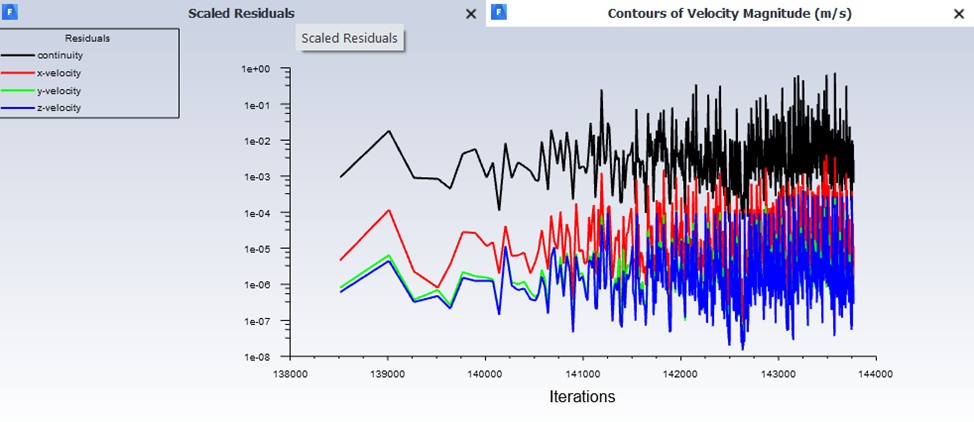
\includegraphics[width=1\linewidth]{../Assets/scaledResiduals}
		\caption{Scaled residuals}
		\label{fig:scaledresiduals}
	\end{figure}
	
	For post processing and plotting based on them, the built-in ANSYS CFD-Post tool was used. It is a program for processing the results of calculations, which has a wide range of all the necessary tools: creating animations, graphs, contour distributions of flow parameters, vector fields, streamlines, volumetric rendering, template reports and much more. To analyze the effect of vortex generators on local friction and transfer, different sections were used in different parts of the channel. Some of them are shown on the figure \ref{fig:planesforanalysis}. 
	\begin{figure}[H]
		\centering
		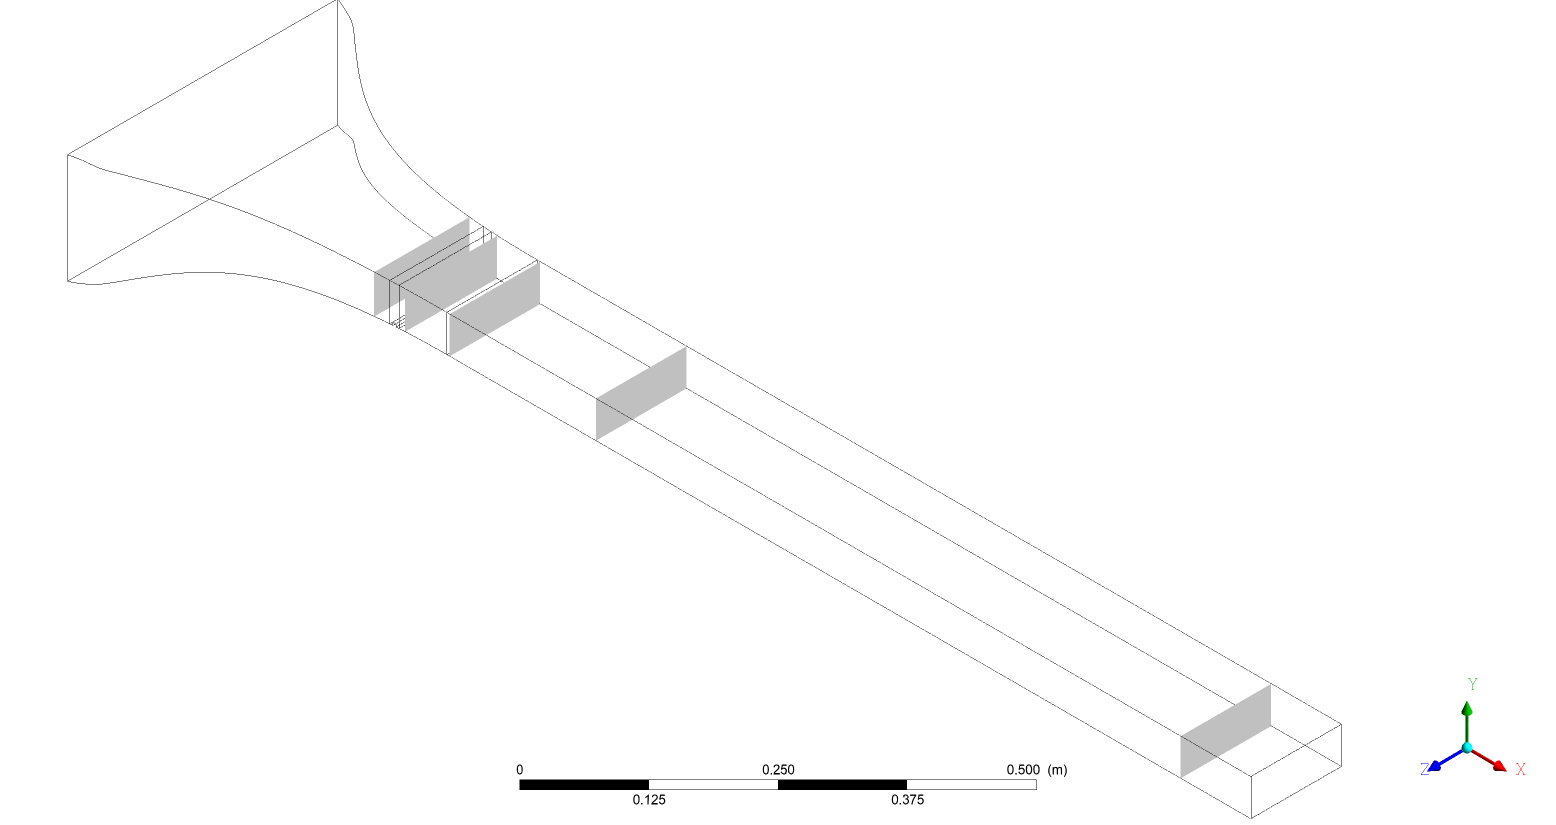
\includegraphics[width=0.9\linewidth]{../Assets/1}
		\caption{Sections for analysis}
		\label{fig:planesforanalysis}
	\end{figure}
	
	The origin of the coordinate axes of the model is located in the center of the channel entrance. Sections were considered at different heights along and at different distances from the entrance to the channel. The table below shows a list of sections, their location and description. Images in applications have names based on the table.
	\begin{table}[H]
		\begin{center}
			\begin{tabular}{|c|c|c|c|}
				\hline
				Label & Plane & Position & Description\\
				\hline
				PlaneXY & XY & Z = 0 & along the whole channel\\
				\hline
				PlaneYZ300 & YZ & X = 300 & in front of the barrier\\
				\hline
				PlaneYZ340 & YZ & X = 340 & after the barrier\\
				\hline
				PlaneYZ400 & YZ & X = 400 & begin of the straight section\\
				\hline
				PlaneYZ600 & YZ & X = 600 & further down the channel\\
				\hline
				PlaneYZ1400 & YZ & X = 1400 & at the exit of the channel\\
				\hline
				PlaneXZ0 & XZ & Y = 0 & above the boundary layer\\
				\hline
				PlaneXZ20M & XZ & Y = -20 & above the barrier\\
				\hline
				PlaneXZ23М & XZ & Y = -23 & at the barrier level\\
				\hline
			\end{tabular}
		\end{center}
		\label{tbl:sections}
		\caption{List of sections}
	\end{table}
	
\subsection{Influence on local friction and transport}
	Further, for the convenience of describing the results and their evaluation, several points are presented on various parameters.
\subsubsection{Velocity}
	Let's start with velocity. According to the obtained sections, the contours of average velocity were constructed for various time intervals.
	\begin{figure}[H]
		\centering
		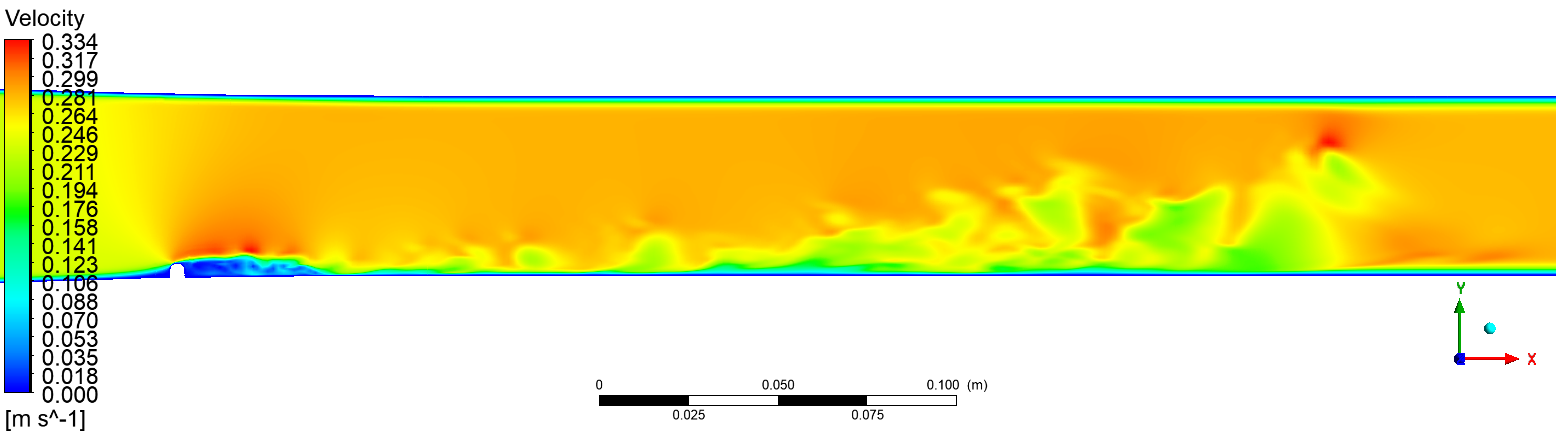
\includegraphics[width=1\linewidth]{../Assets/T16_Velocity_ContourXY}
		\caption{Velocity in longitudinal section XY, t = 1.6 c}
		\label{fig:t16velocitycontourxy}
	\end{figure}
	As can be seen from the figure along the channel, the velocity immediately behind the barrier and at its level approached zero. And over the wire has increased significantly. Due to such abrupt changes in speed, vortex structures are formed, the speed of which is clearly visible in these images. These vortex formations can also be seen in figure \ref{fig:T16VelocityContourYZ}. At the end of channel($x = 1400$) velocity is unchanged because the flow has not reached the given section.
	\begin{figure}[H]
		\begin{subfigure}{.5\textwidth}
			\centering
			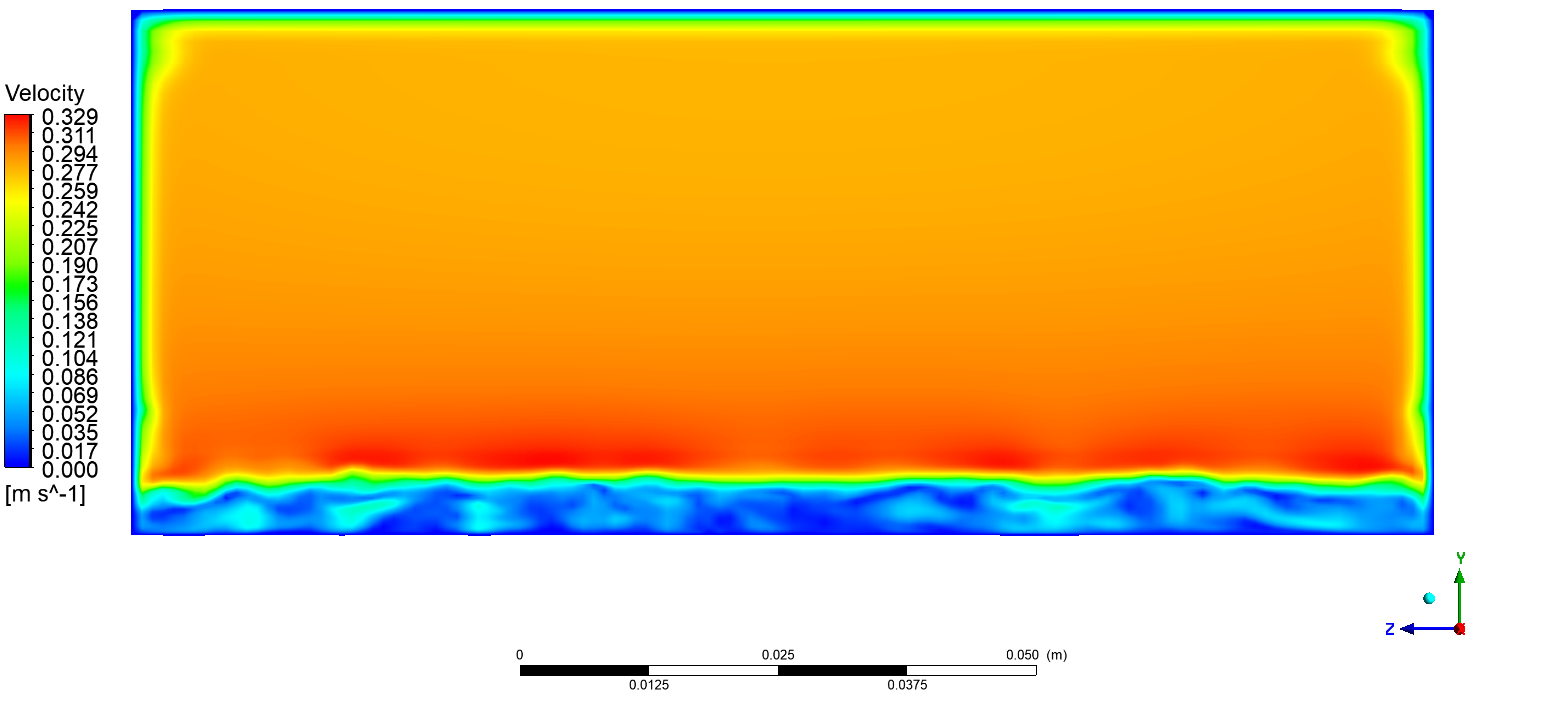
\includegraphics[width=1.1\linewidth]{../Assets/T16_Velocity_ContourYZ340}
			\caption{PlaneYZ340}
			\label{fig:T16VelocityContourYZ340}
		\end{subfigure}%
		\begin{subfigure}{.5\textwidth}
			\centering
			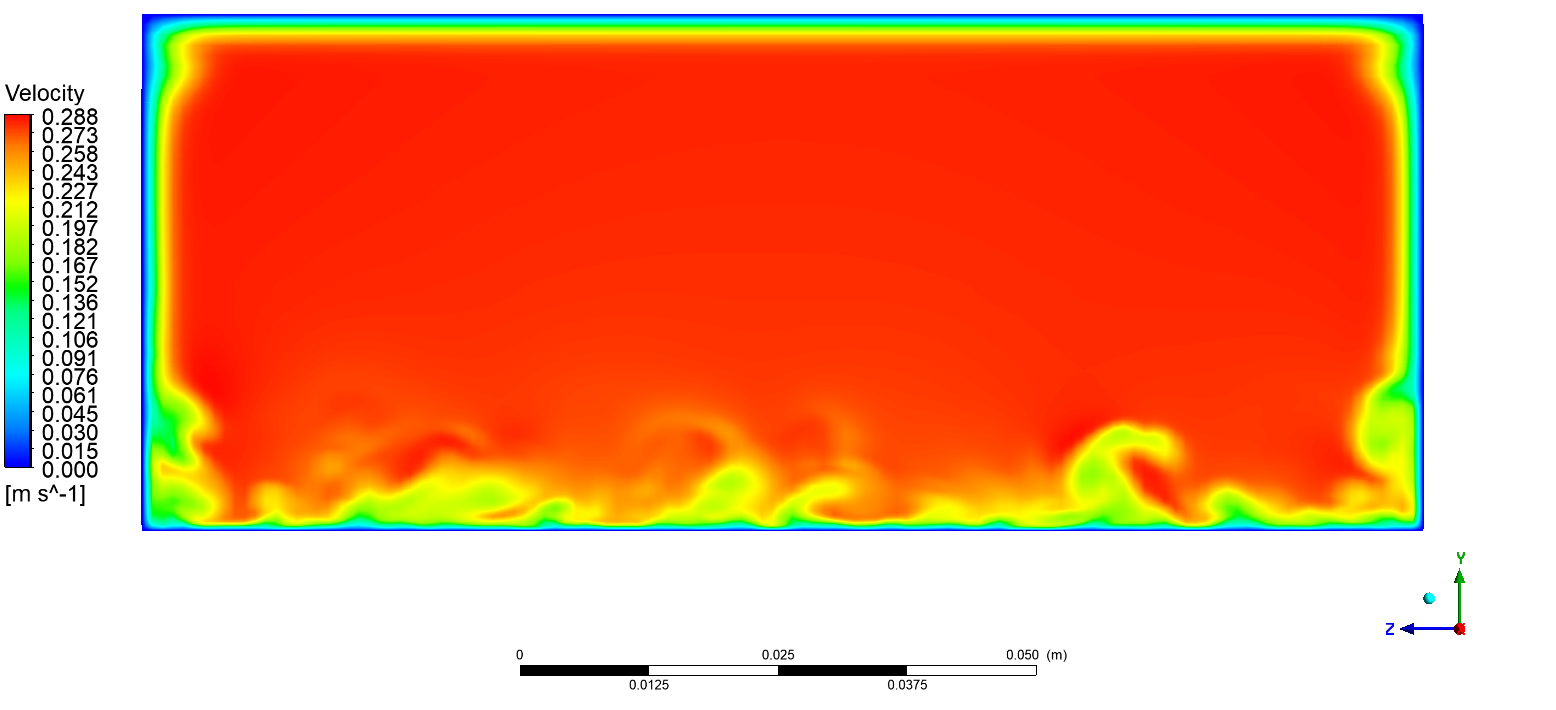
\includegraphics[width=1.1\linewidth]{../Assets/T16_Velocity_ContourYZ400}
			\caption{PlaneYZ400}
			\label{fig:T16VelocityContourYZ400}
		\end{subfigure}
		\\
		\begin{subfigure}{.5\textwidth}
			\centering
			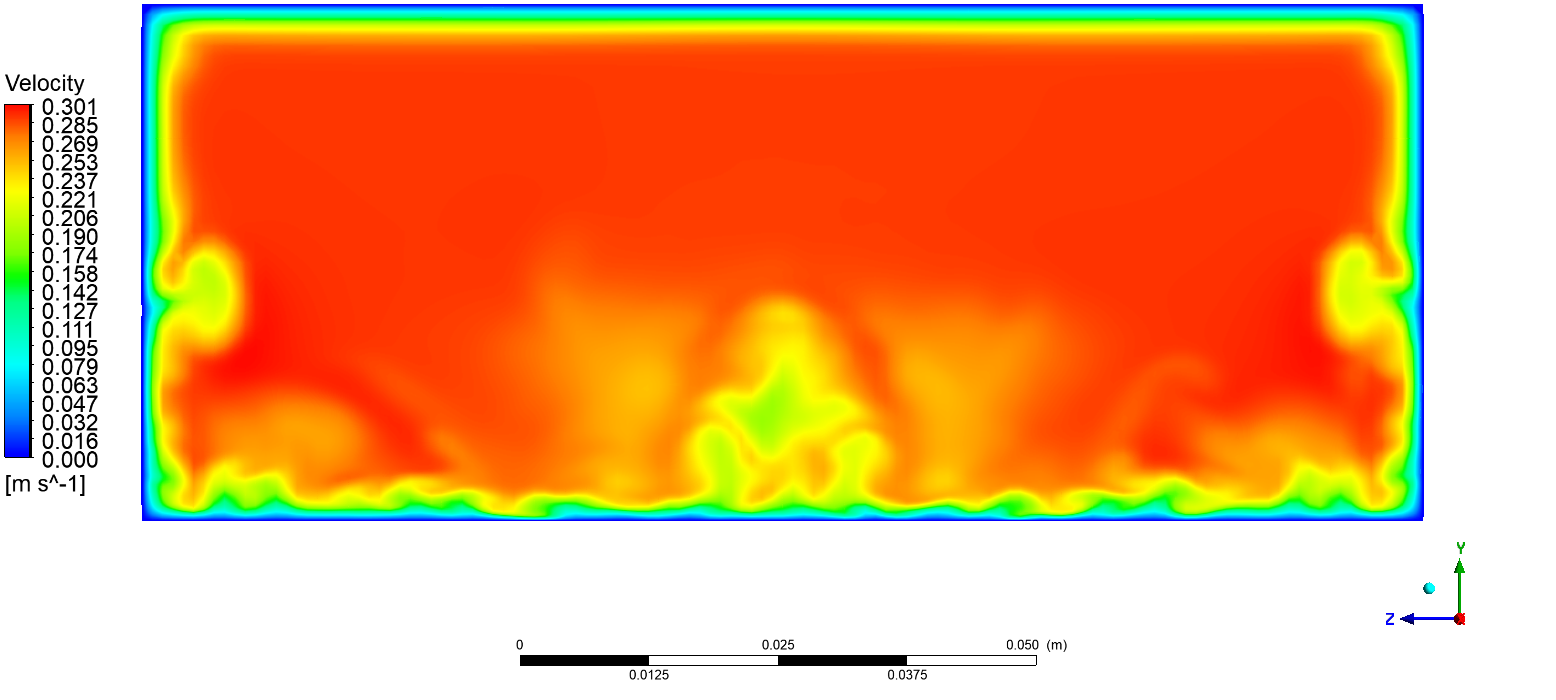
\includegraphics[width=1.1\linewidth]{../Assets/T16_Velocity_ContourYZ600}
			\caption{PlaneYZ600}
			\label{fig:T16VelocityContourYZ600}
		\end{subfigure}%
		\begin{subfigure}{.5\textwidth}
			\centering
			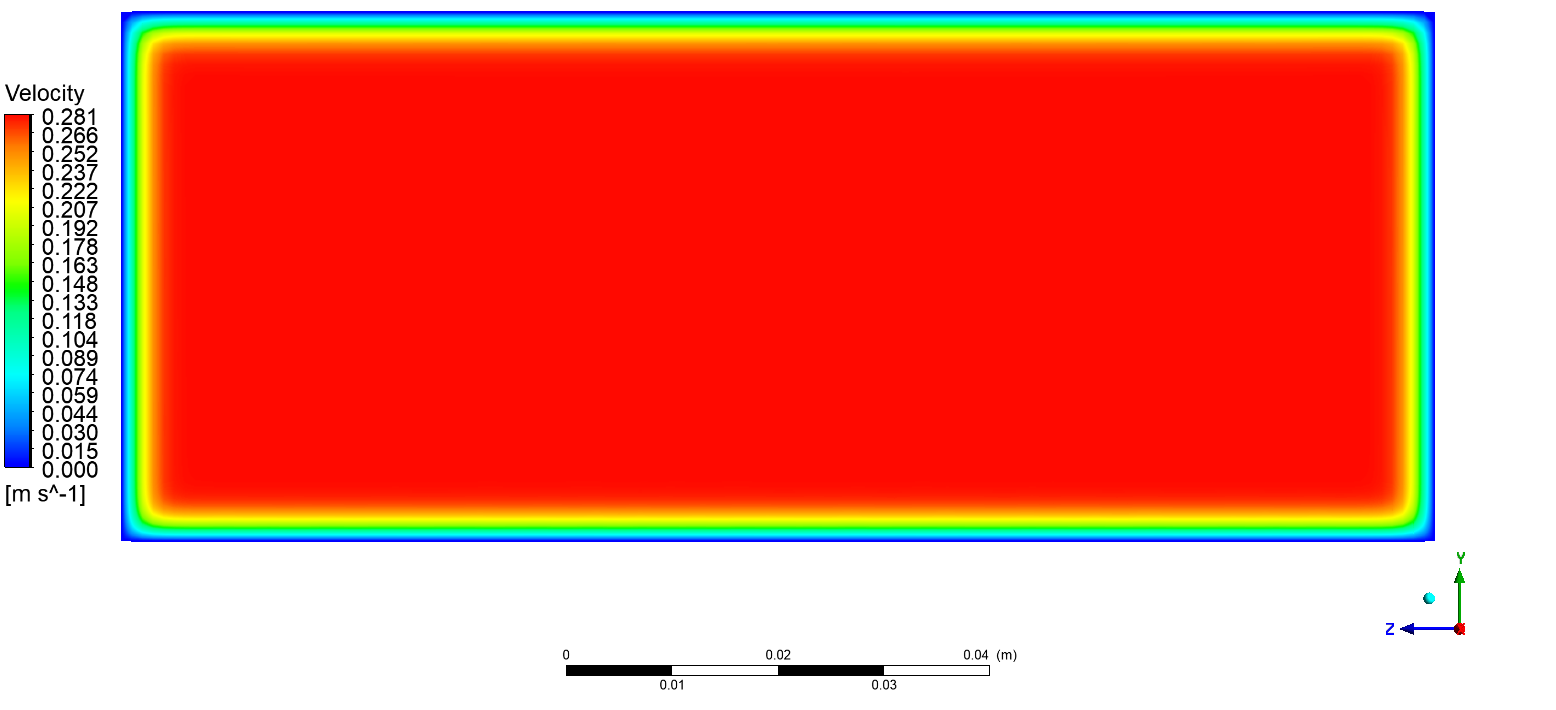
\includegraphics[width=1.1\linewidth]{../Assets/T16_Velocity_ContourYZ1400}
			\caption{PlaneYZ1400}
			\label{fig:T16VelocityContourYZ1400}
		\end{subfigure}
		\caption{Velocity in cross sections at t = 1.6 s}
		\label{fig:T16VelocityContourYZ}
	\end{figure}
	After a while, the flow stabilized a little bit. But in boundary layer there are a lot of turbulent structures.
	\begin{figure}[H]
		\centering
		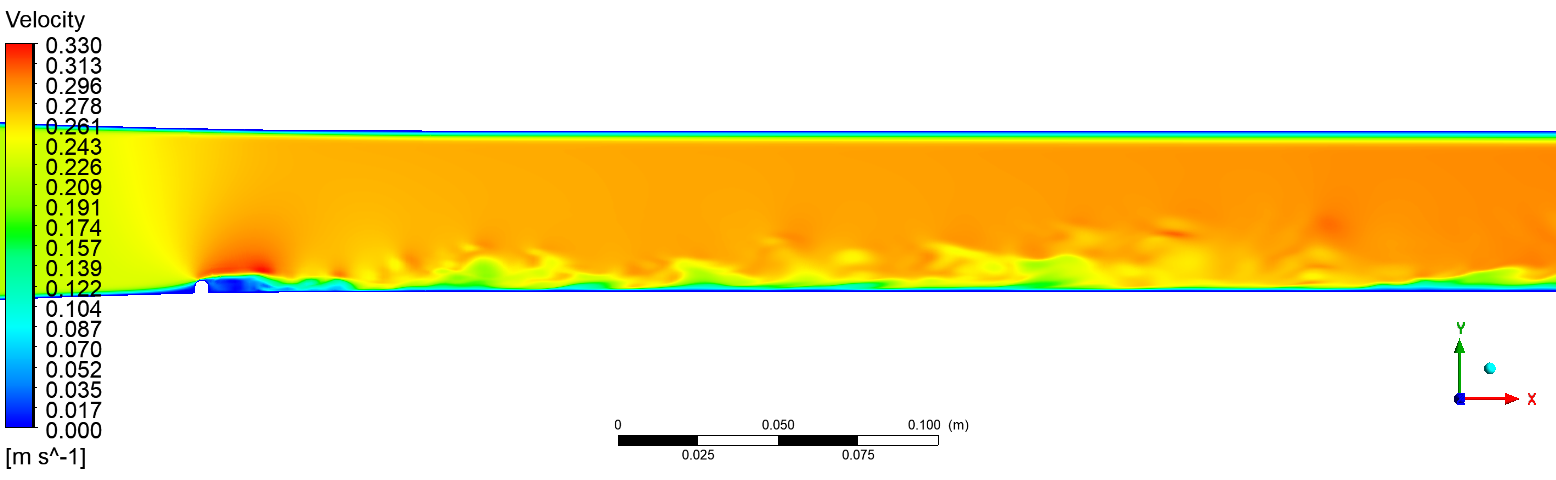
\includegraphics[width=1\linewidth]{../Assets/T96_Velocity_ContourXY}
		\caption{Longitudinal velocity in XY, t = 9.6 s}
		\label{fig:t96velocitycontourxy}
	\end{figure}
	By the time t = 9.6 s, the vortex structure of the channel became less visible and large eddies were transformed into small ones.
	Let us consider more detail velocity in cross sections at time t = 9.6 s. As seen in the picture \ref{fig:T96VelocityContourYZ} the formed vortices gradually decay to Kolmagorov scale vortices and dissipate into energy.
	\begin{figure}[H]
		\begin{subfigure}{.5\textwidth}
			\centering
			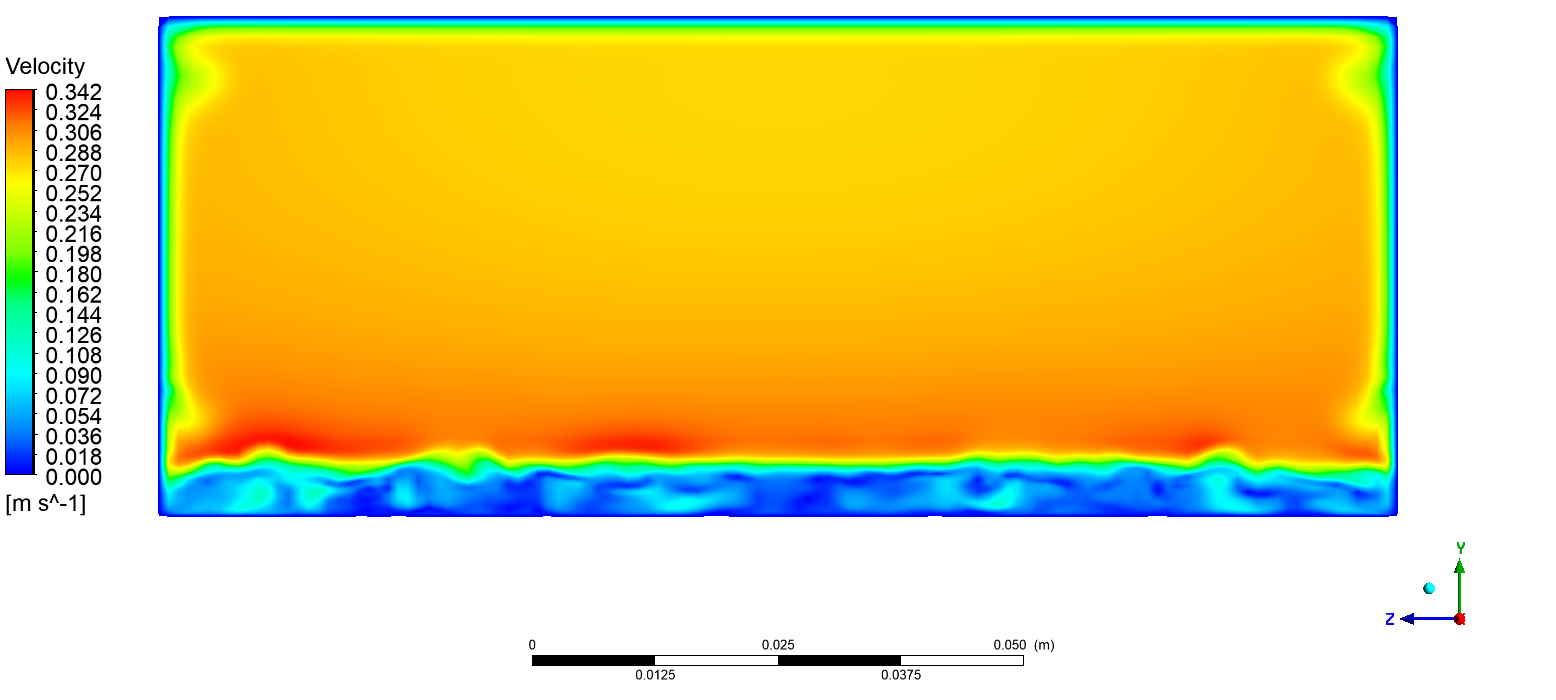
\includegraphics[width=1.1\linewidth]{../Assets/T96_Velocity_ContourYZ340}
			\caption{PlaneYZ340}
			\label{fig:T96VelocityContourYZ340}
		\end{subfigure}%
		\begin{subfigure}{.5\textwidth}
			\centering
			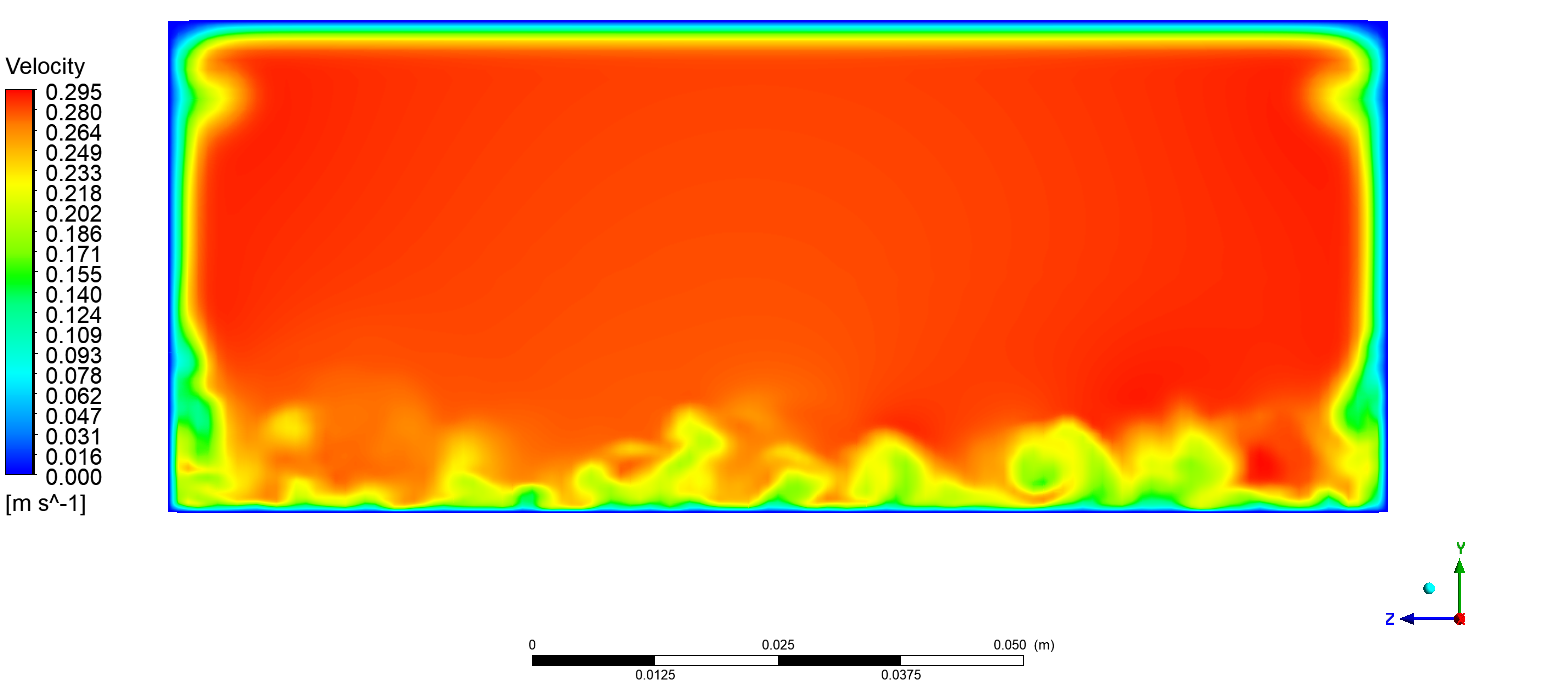
\includegraphics[width=1.1\linewidth]{../Assets/T96_Velocity_ContourYZ400}
			\caption{PlaneYZ400}
			\label{fig:T96VelocityContourYZ400}
		\end{subfigure}
		\\
		\begin{subfigure}{.5\textwidth}
			\centering
			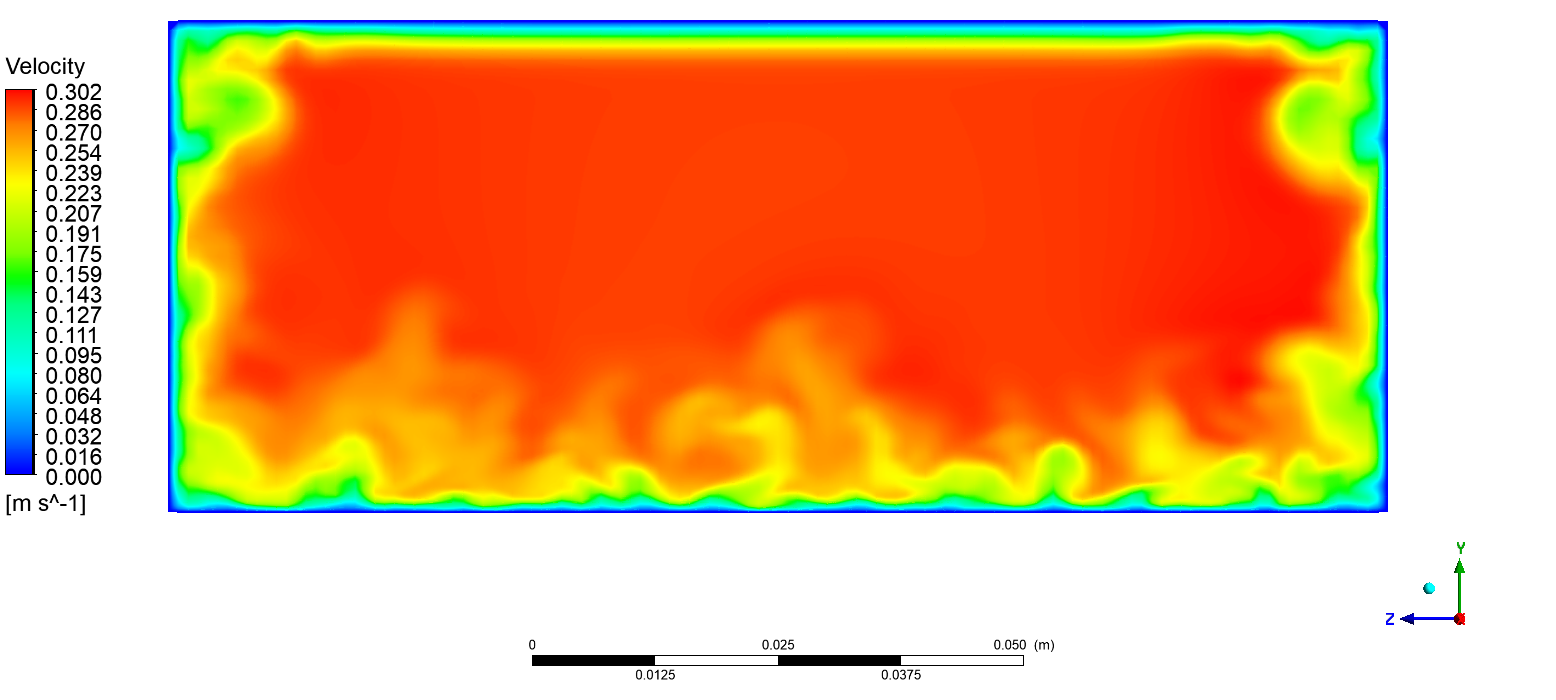
\includegraphics[width=1.1\linewidth]{../Assets/T96_Velocity_ContourYZ600}
			\caption{PlaneYZ600}
			\label{fig:T96VelocityContourYZ600}
		\end{subfigure}%
		\begin{subfigure}{.5\textwidth}
			\centering
			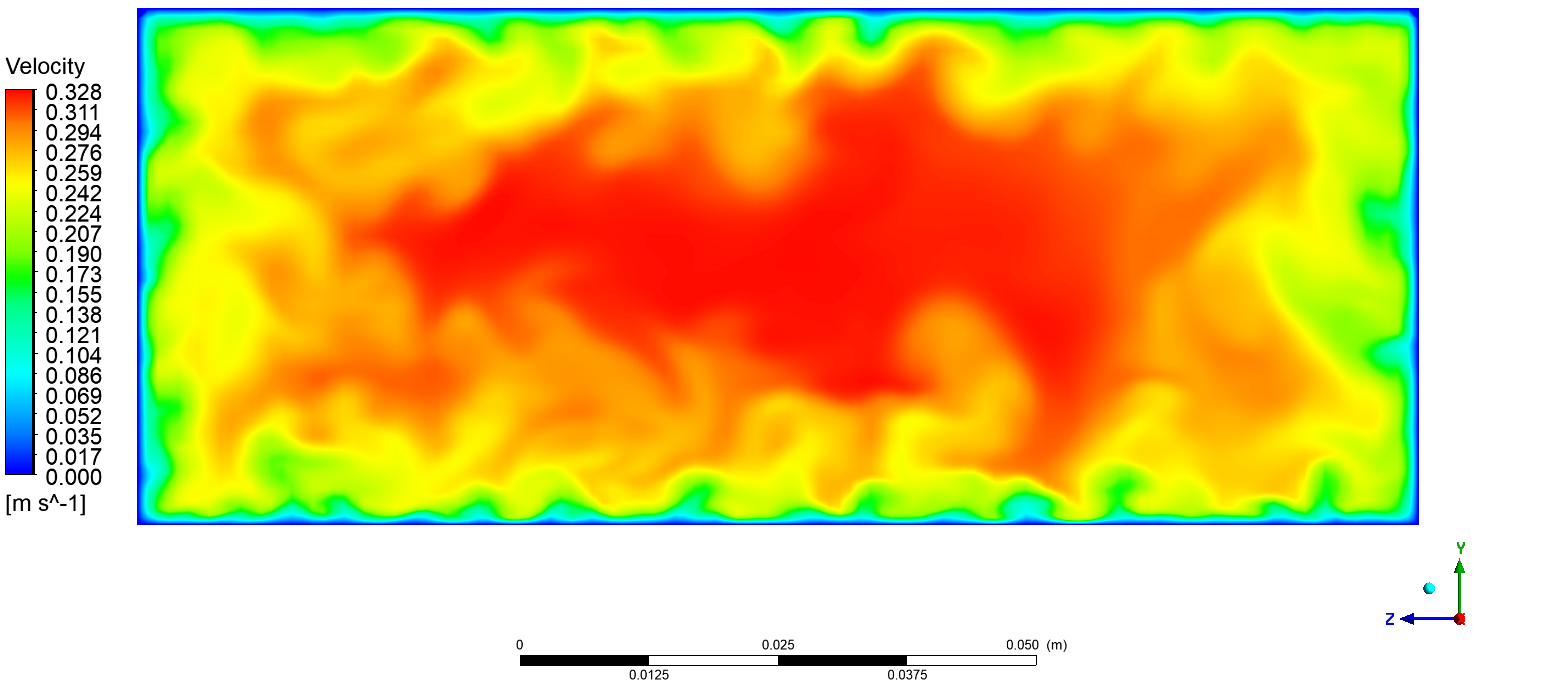
\includegraphics[width=1.1\linewidth]{../Assets/T96_Velocity_ContourYZ1400}
			\caption{PlaneYZ1400}
			\label{fig:T96VelocityContourYZ1400}
		\end{subfigure}
		\caption{Velocity in cross sections at t = 9.6 s}
		\label{fig:T96VelocityContourYZ}
	\end{figure}
	\newpage
	At picture \ref{fig:T16VelocityContourXZ} we can see how turbulent structures generates from different heights. Also we see some big vortices on the right side of pictures.
	\begin{figure}[H]
		\begin{subfigure}{1\textwidth}
			\centering
			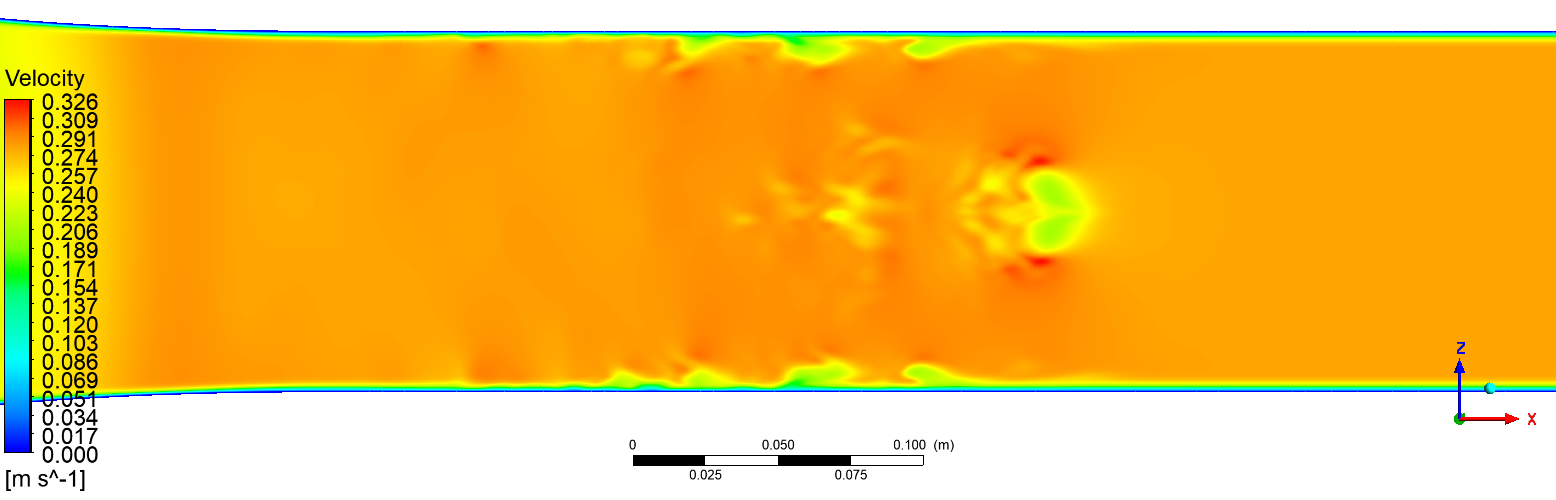
\includegraphics[width=1\linewidth]{../Assets/T16_Velocity_ContourXZ0}
			\caption{PlaneXZ0}
			\label{fig:T16VelocityContourXZ0}
		\end{subfigure}%
		\\
		\begin{subfigure}{1\textwidth}
			\centering
			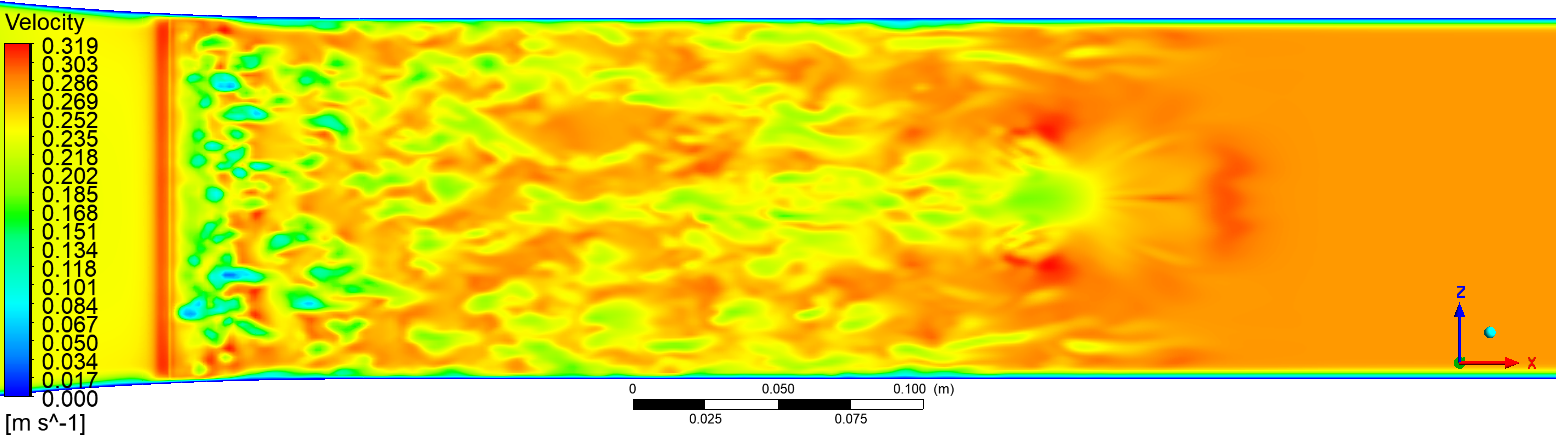
\includegraphics[width=1\linewidth]{../Assets/T16_Velocity_ContourXZ20M}
			\caption{PlaneXZ20M}
			\label{fig:T16VelocityContourXZ20M}
		\end{subfigure}%
		\\
		\begin{subfigure}{1\textwidth}
			\centering
			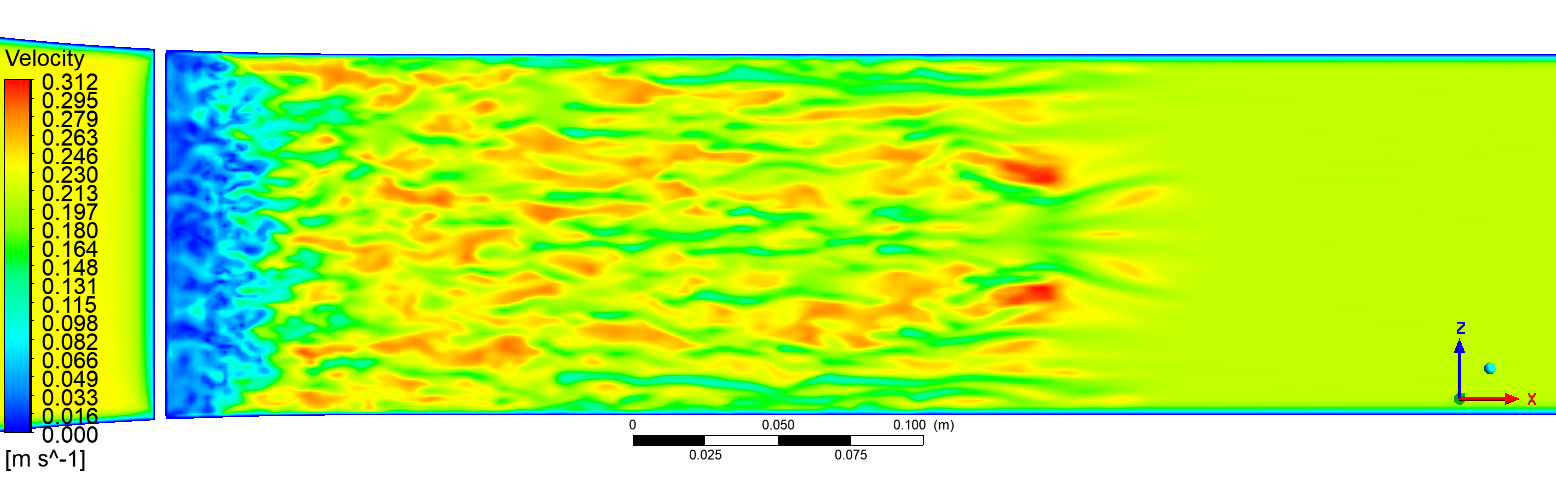
\includegraphics[width=1\linewidth]{../Assets/T16_Velocity_ContourXZ23M}
			\caption{PlaneXZ23M}
			\label{fig:T16VelocityContourXZ23M}
		\end{subfigure}
		\caption{Speed in longitudinal sections XZ at t = 1.6 s}
		\label{fig:T16VelocityContourXZ}
	\end{figure}
	\newpage
	After some time big structures divided into numerous number of small size. So we can see them on picture \ref{fig:T76VelocityContourXZ}.
	\begin{figure}[H]
		\begin{subfigure}{1\textwidth}
			\centering
			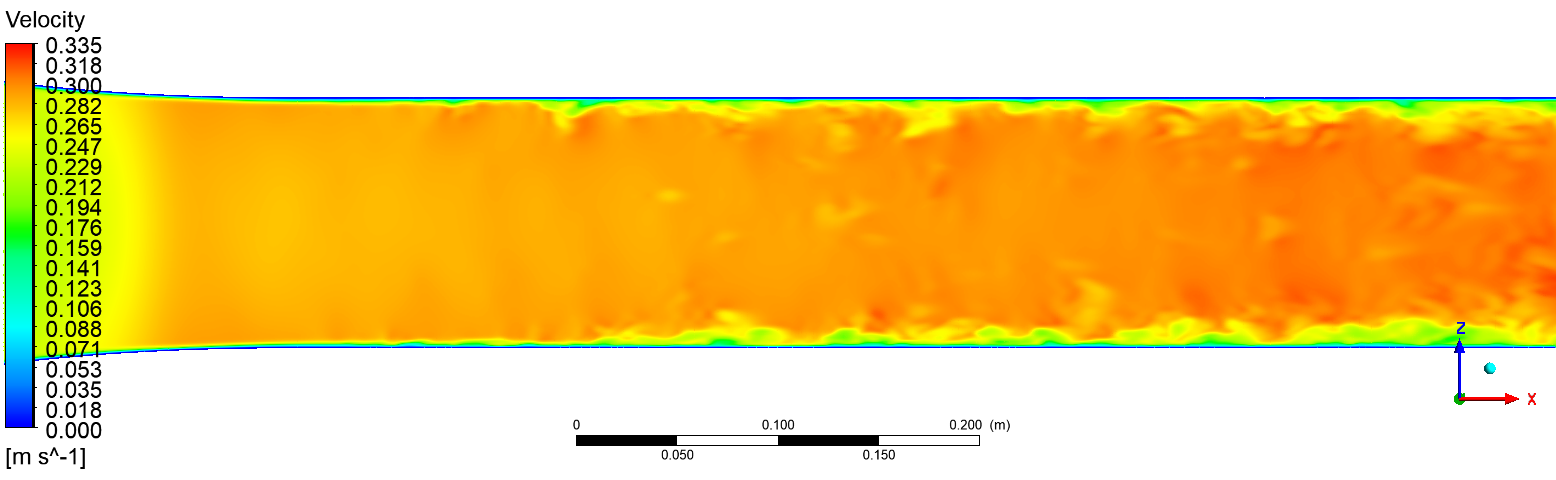
\includegraphics[width=1\linewidth]{../Assets/T76_Velocity_ContourXZ0}
			\caption{PlaneXZ0}
			\label{fig:T76VelocityContourXZ0}
		\end{subfigure}%
		\\
		\begin{subfigure}{1\textwidth}
			\centering
			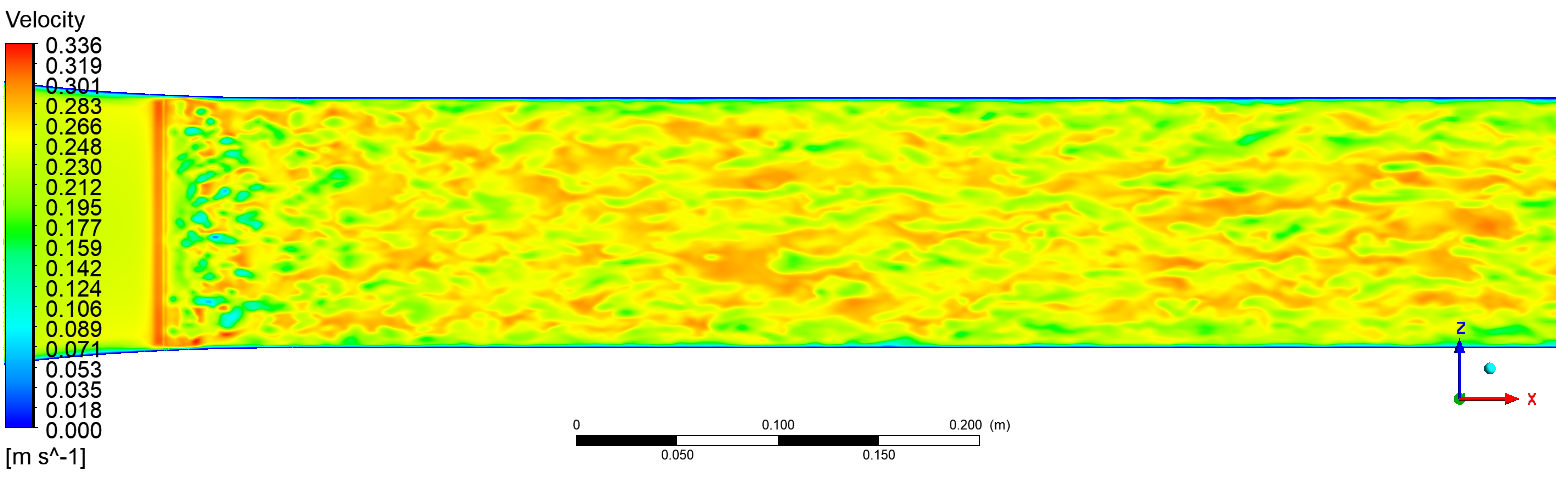
\includegraphics[width=1\linewidth]{../Assets/T76_Velocity_ContourXZ20M}
			\caption{PlaneXZ20M}
			\label{fig:T76VelocityContourXZ20M}
		\end{subfigure}%
		\\
		\begin{subfigure}{1\textwidth}
			\centering
			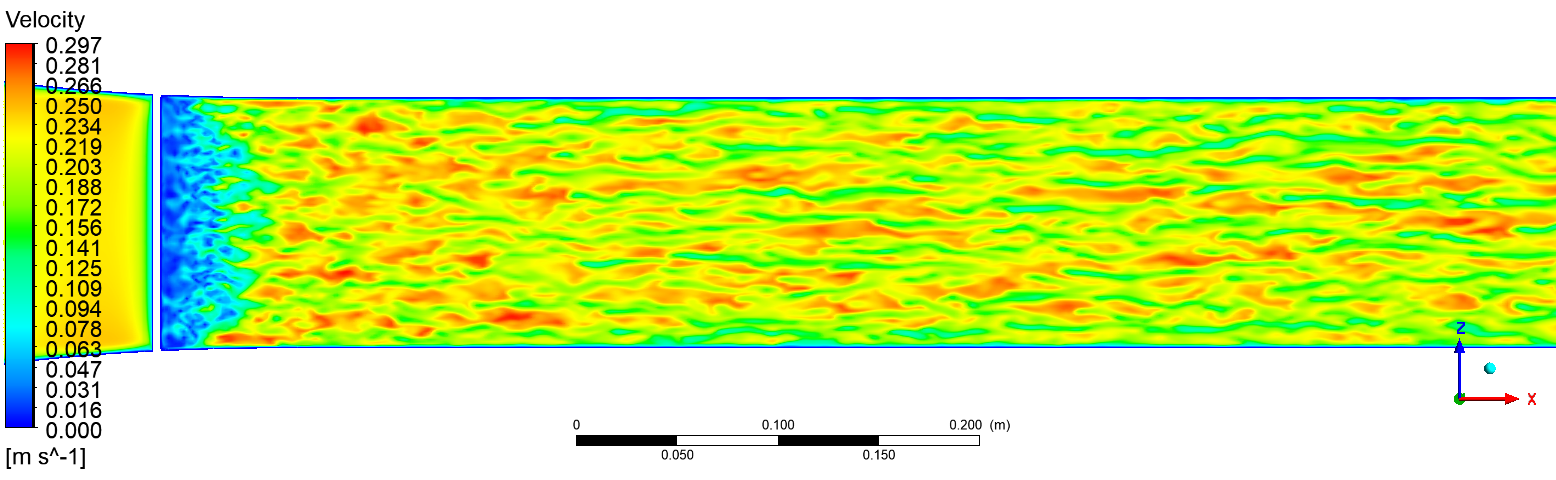
\includegraphics[width=1\linewidth]{../Assets/T76_Velocity_ContourXZ23M}
			\caption{PlaneXZ23M}
			\label{fig:T76VelocityContourXZ23M}
		\end{subfigure}
		\caption{Speed in longitudinal sections XZ at t = 7.6 s}
		\label{fig:T76VelocityContourXZ}
	\end{figure}
	\newpage
\subsubsection{Friction coefficient}
	In order to obtain friction coefficient data for plotting, the necessary sections were built in Ansys Fluent. They divide the channel lengthwise into 3 parts ($z_1 = -31, z_2 = 0, z_3 = 31$). After that, the built-in tools exported the data to $.csv$ files. Further, with the help of MS Excel, the data concerning the boundary layer were selected. And finally, plots are generated in gnuplot. Four time periods were evaluated($t_1 = 0.6, t_2 = 3.6, t_3 = 7.6, t_4 = 10.6$). The plots show the dependence of $C_f$ on the coordinate $x$. 
	
	The first group of images shows changes in the friction coefficient in the cross section at $z = 0$. From the rectilinear section on the graph, one can understand to which section of the channel the liquid has reached at this point in time. When the fluid flow reaches a barrier, $C_f$ changes abruptly. As we move along the length of the channel, the coefficient decreases. This is due to a decrease in the influence of vortex structures on the boundary layer.
	\begin{figure}[H]
		\begin{subfigure}{.5\textwidth}
			\centering
			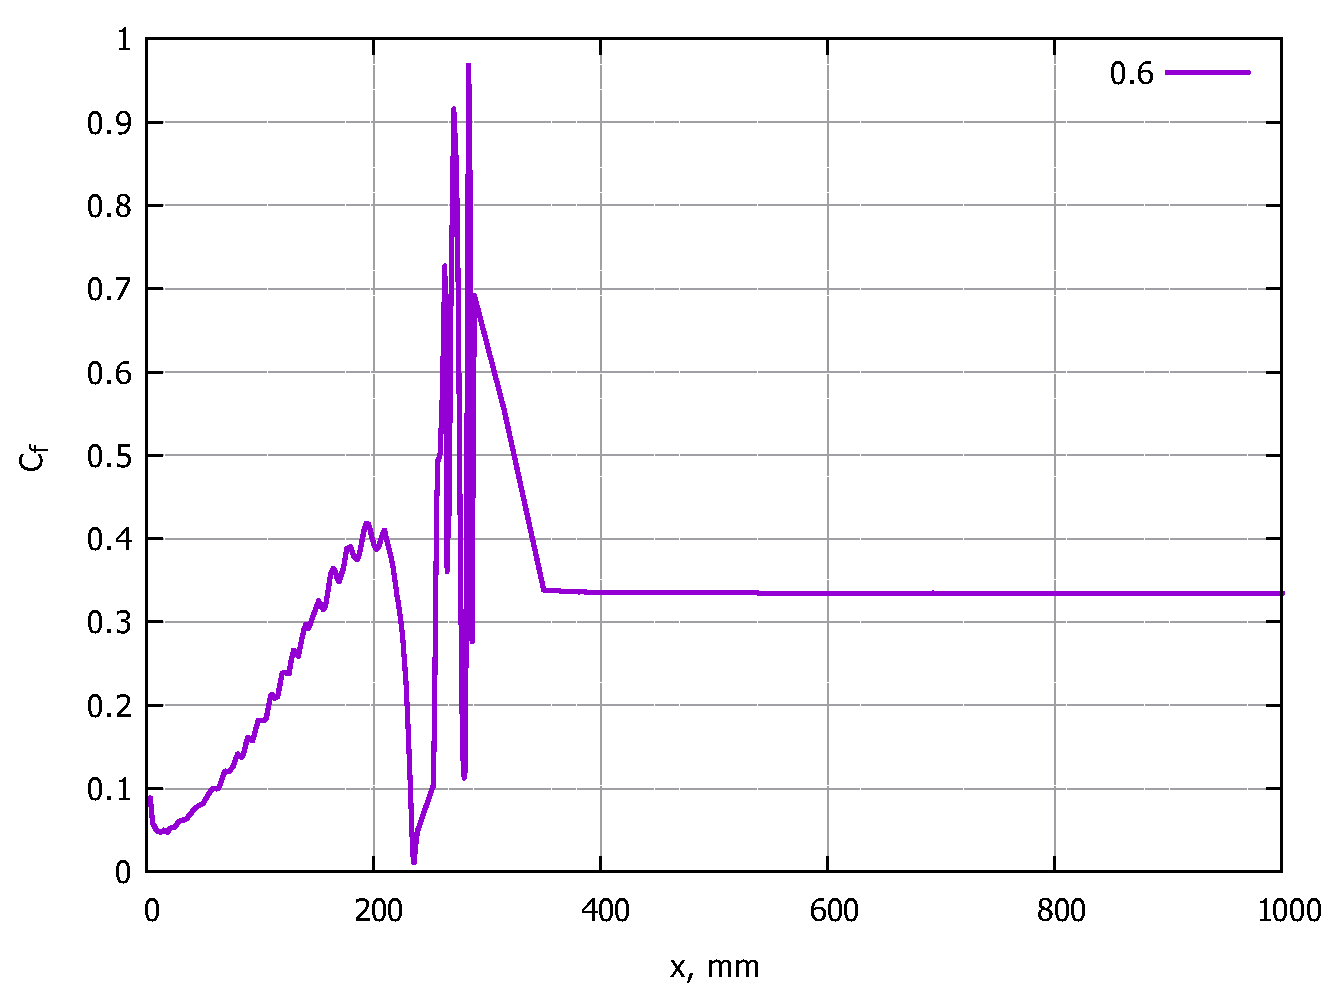
\includegraphics[width=1\linewidth]{../Assets/Cf-T06}
			\caption{t = 0.6 s}
			\label{fig:Cf-T06}
		\end{subfigure}%
		\begin{subfigure}{.5\textwidth}
			\centering
			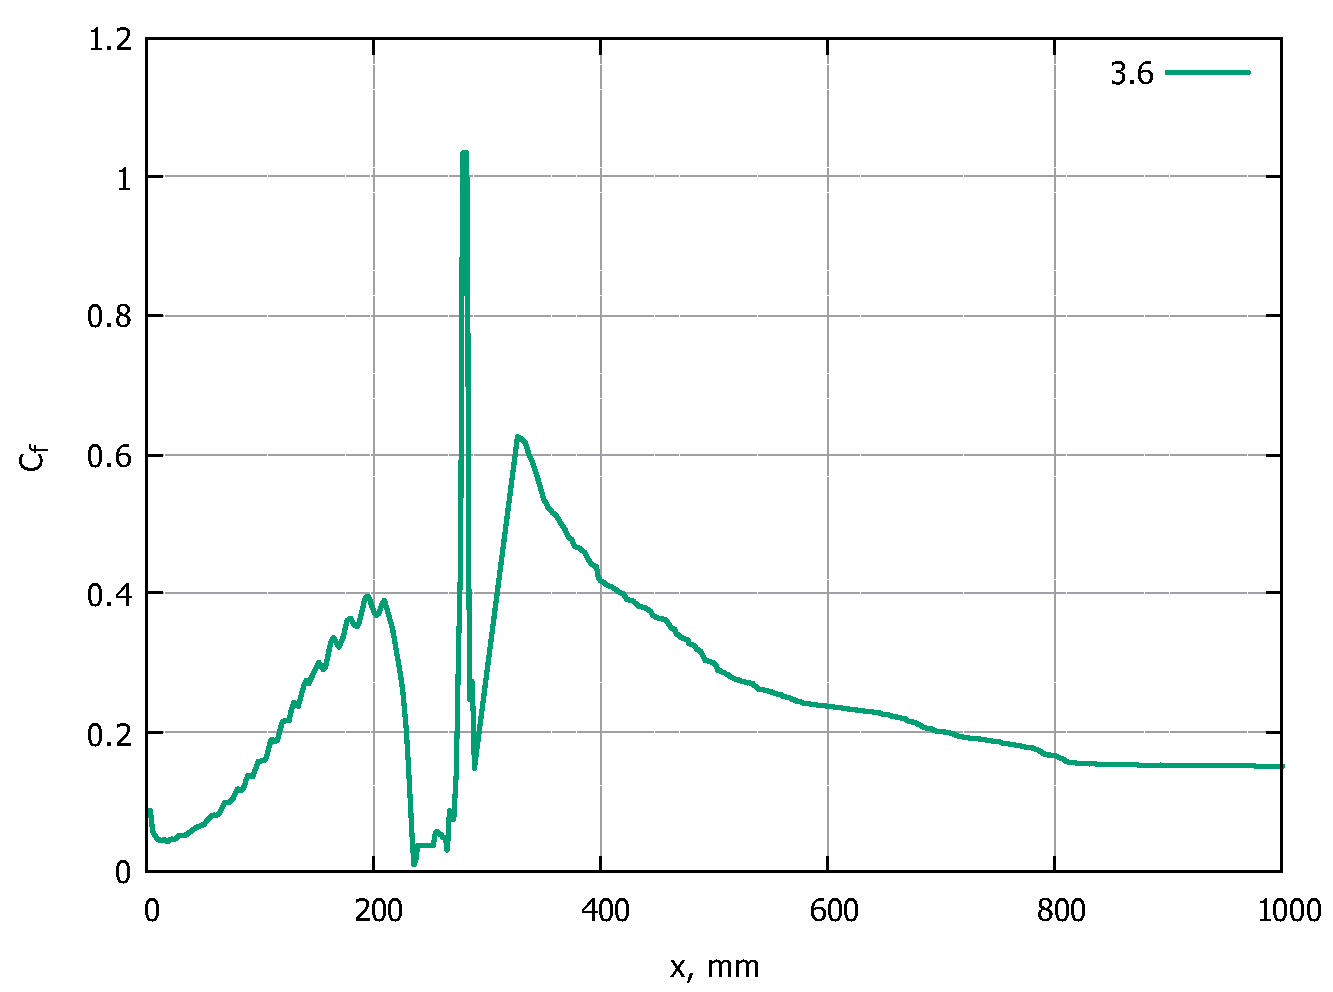
\includegraphics[width=1\linewidth]{../Assets/Cf-T360}
			\caption{t = 3.6 s}
			\label{fig:Cf-T360}
		\end{subfigure}
		\\
		\begin{subfigure}{.5\textwidth}
			\centering
			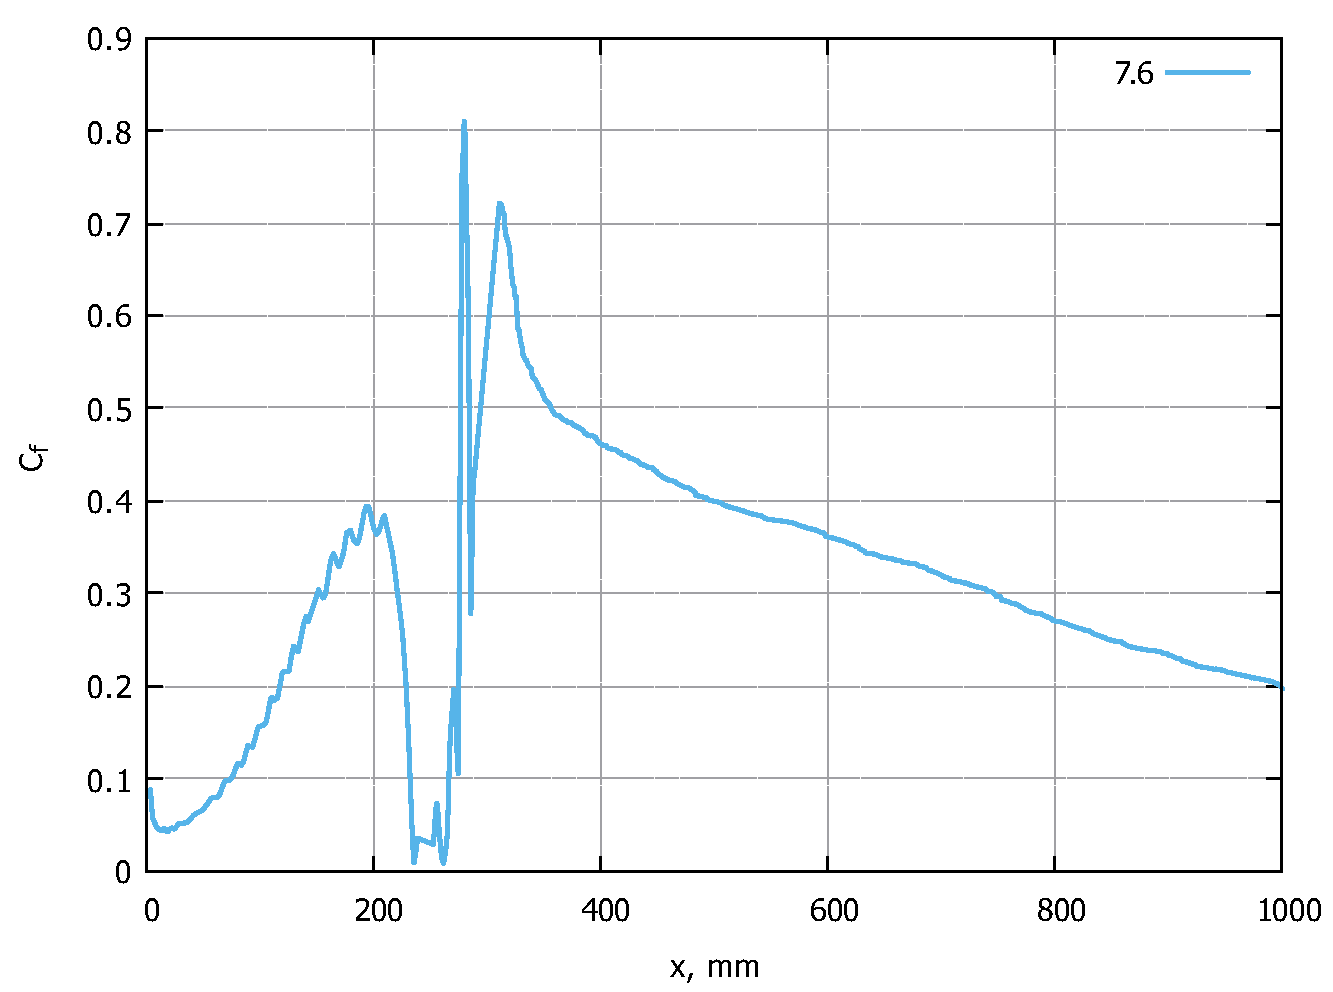
\includegraphics[width=1\linewidth]{../Assets/Cf-T760}
			\caption{t = 7.6 s}
			\label{fig:Cf-T760}
		\end{subfigure}%
		\begin{subfigure}{.5\textwidth}
			\centering
			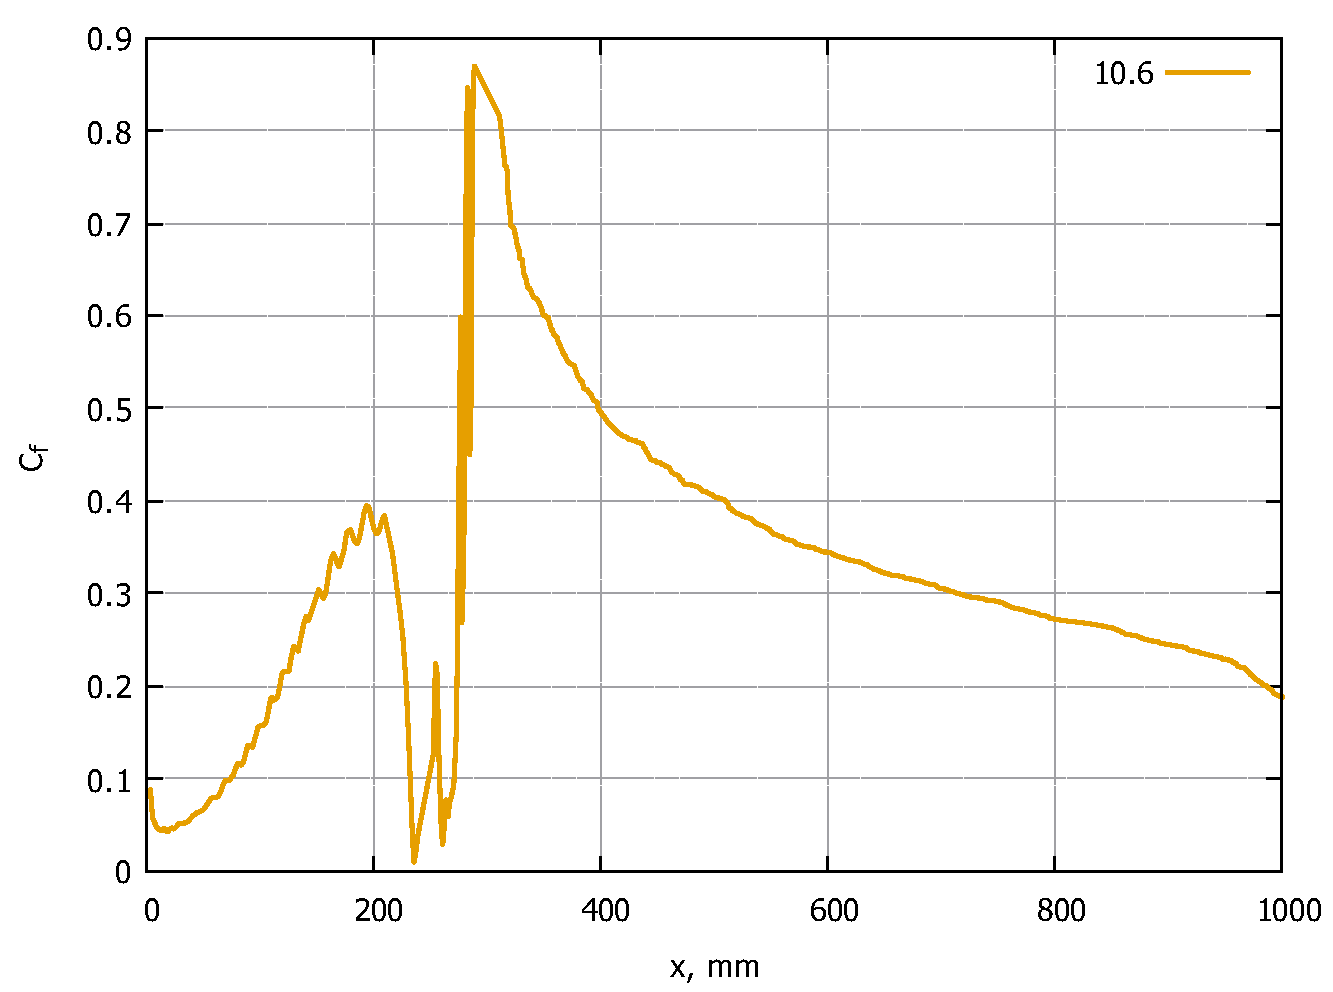
\includegraphics[width=1\linewidth]{../Assets/Cf-T1060}
			\caption{t = 10.6 s}
			\label{fig:Cf-T1060}
		\end{subfigure}
		\caption{Change in the friction coefficient along the length of the channel, z = 0 mm}
		\label{fig:cf}
	\end{figure}
	Further, the second group of images shows the changes in the friction coefficient in the section at $z = -31$. Here, in contrast to the previous section, there are sharper changes in the coefficient behind the barrier.
	\begin{figure}[H]
		\begin{subfigure}{.5\textwidth}
			\centering
			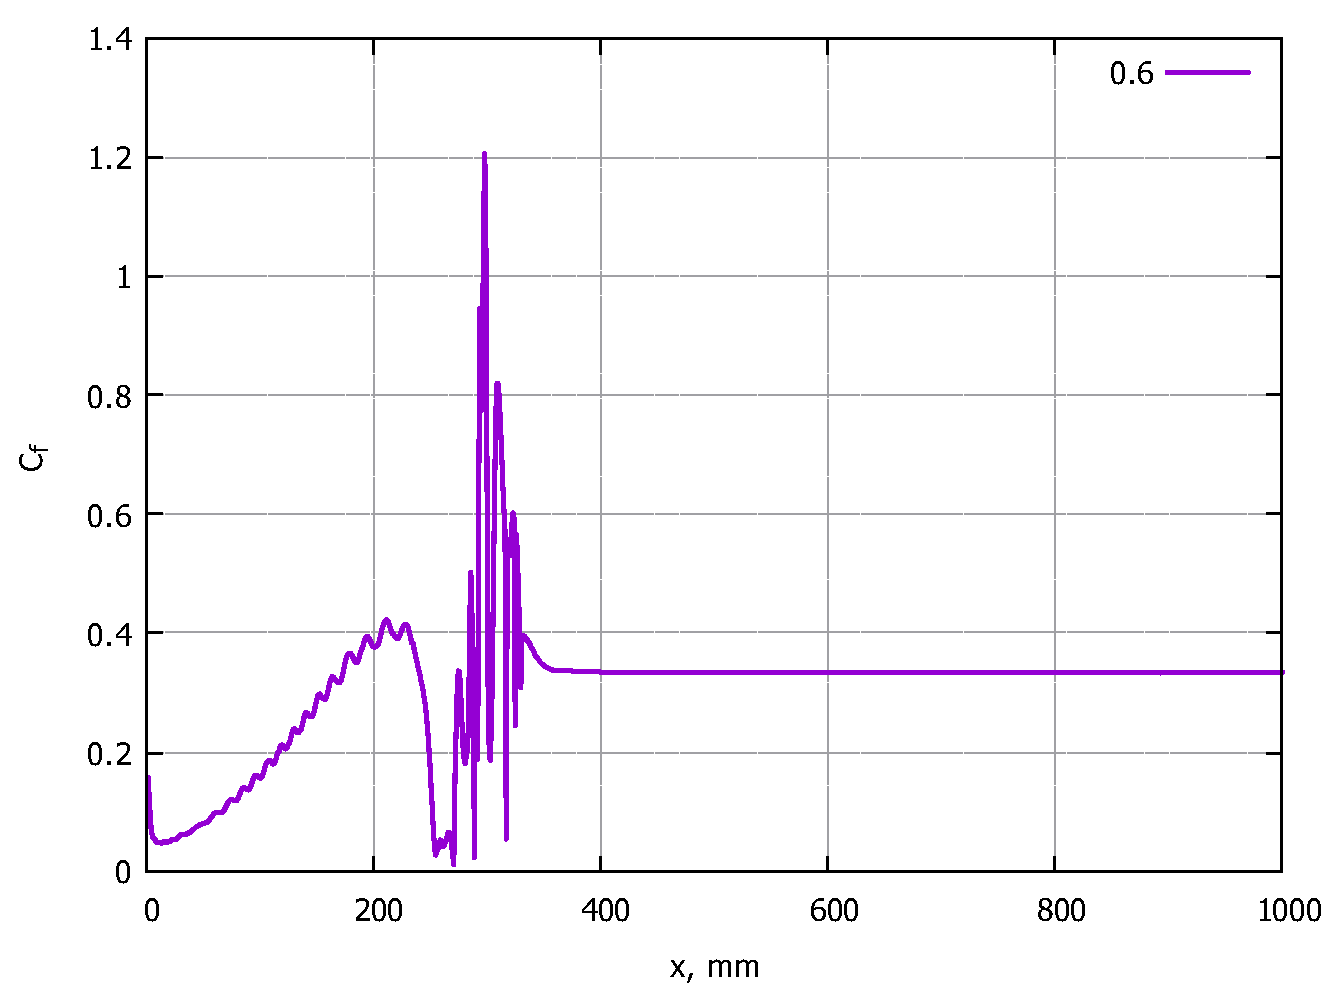
\includegraphics[width=1\linewidth]{../Assets/Cf-T06-31m}
			\caption{t = 0.6 s}
			\label{fig:Cf-T06-31m}
		\end{subfigure}%
		\begin{subfigure}{.5\textwidth}
			\centering
			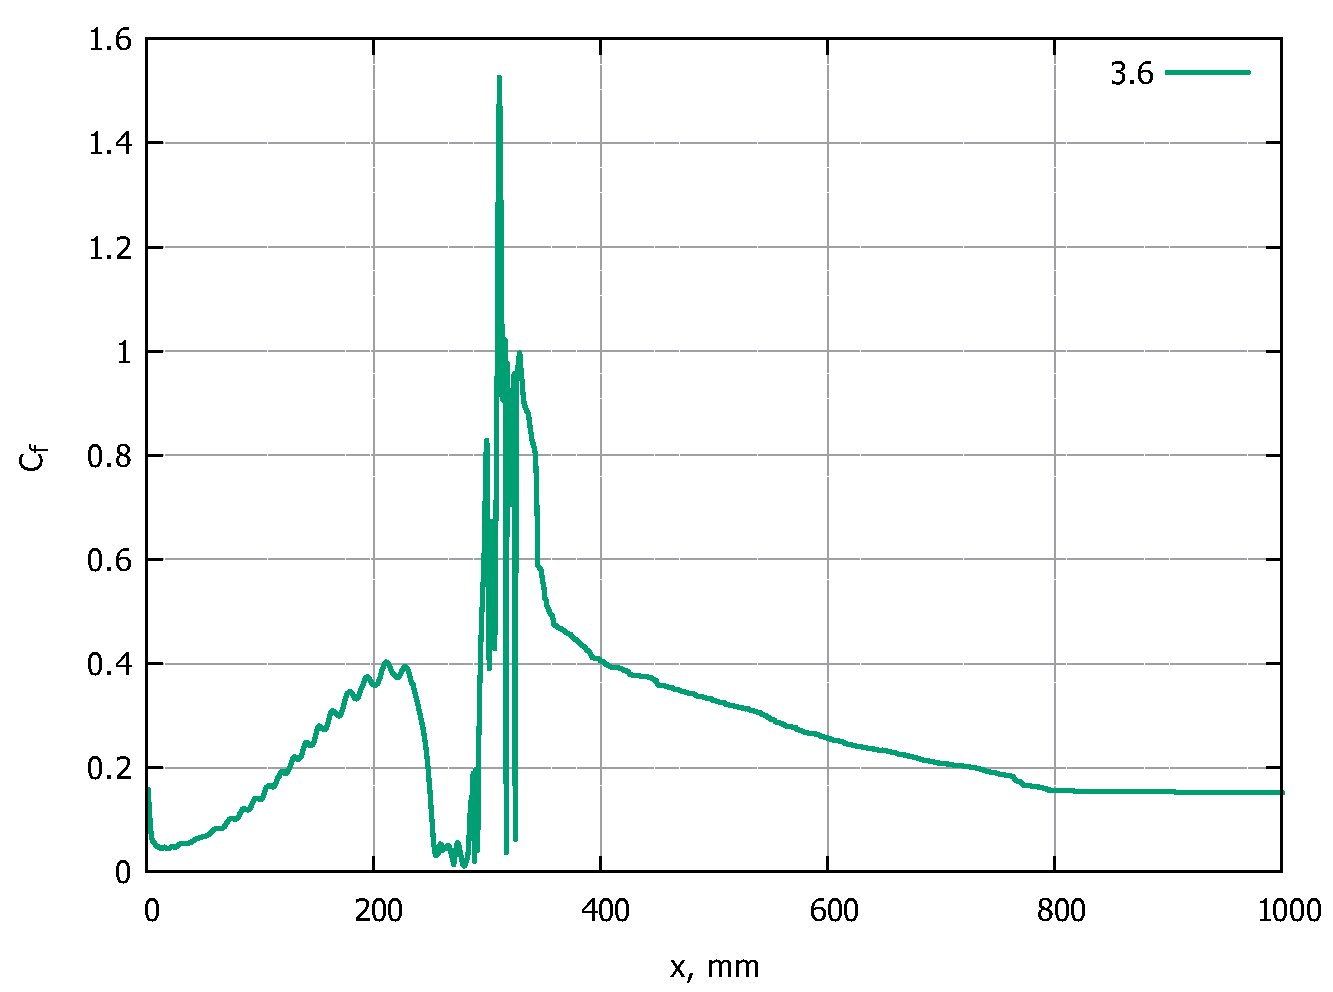
\includegraphics[width=1\linewidth]{../Assets/Cf-T360-31m}
			\caption{t = 3.6 s}
			\label{fig:Cf-T360-31m}
		\end{subfigure}
		\\
		\begin{subfigure}{.5\textwidth}
			\centering
			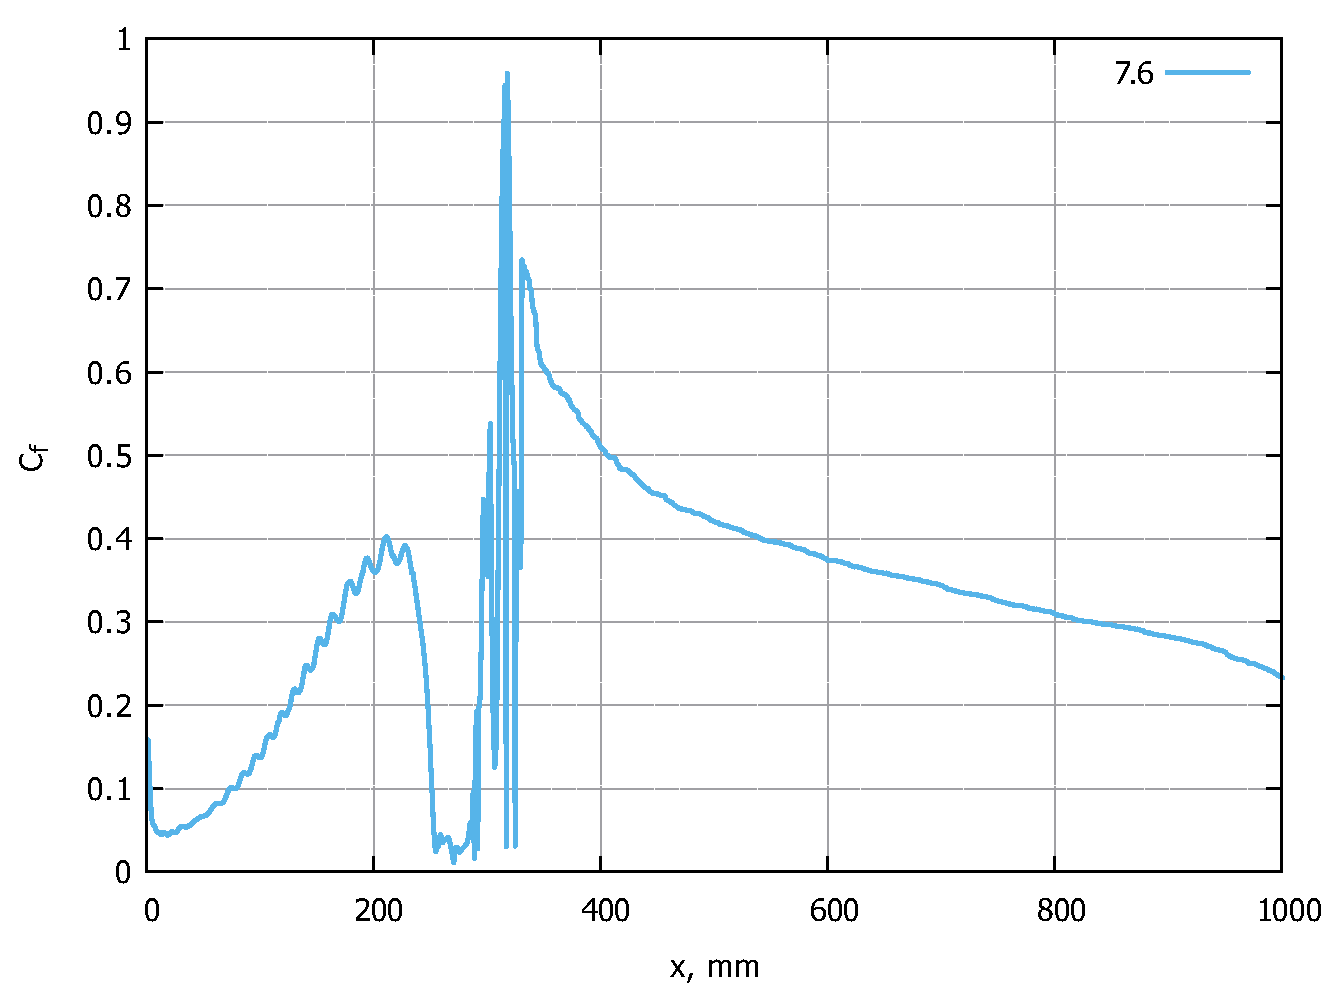
\includegraphics[width=1\linewidth]{../Assets/Cf-T760-31m}
			\caption{t = 7.6 s}
			\label{fig:Cf-T760-31m}
		\end{subfigure}%
		\begin{subfigure}{.5\textwidth}
			\centering
			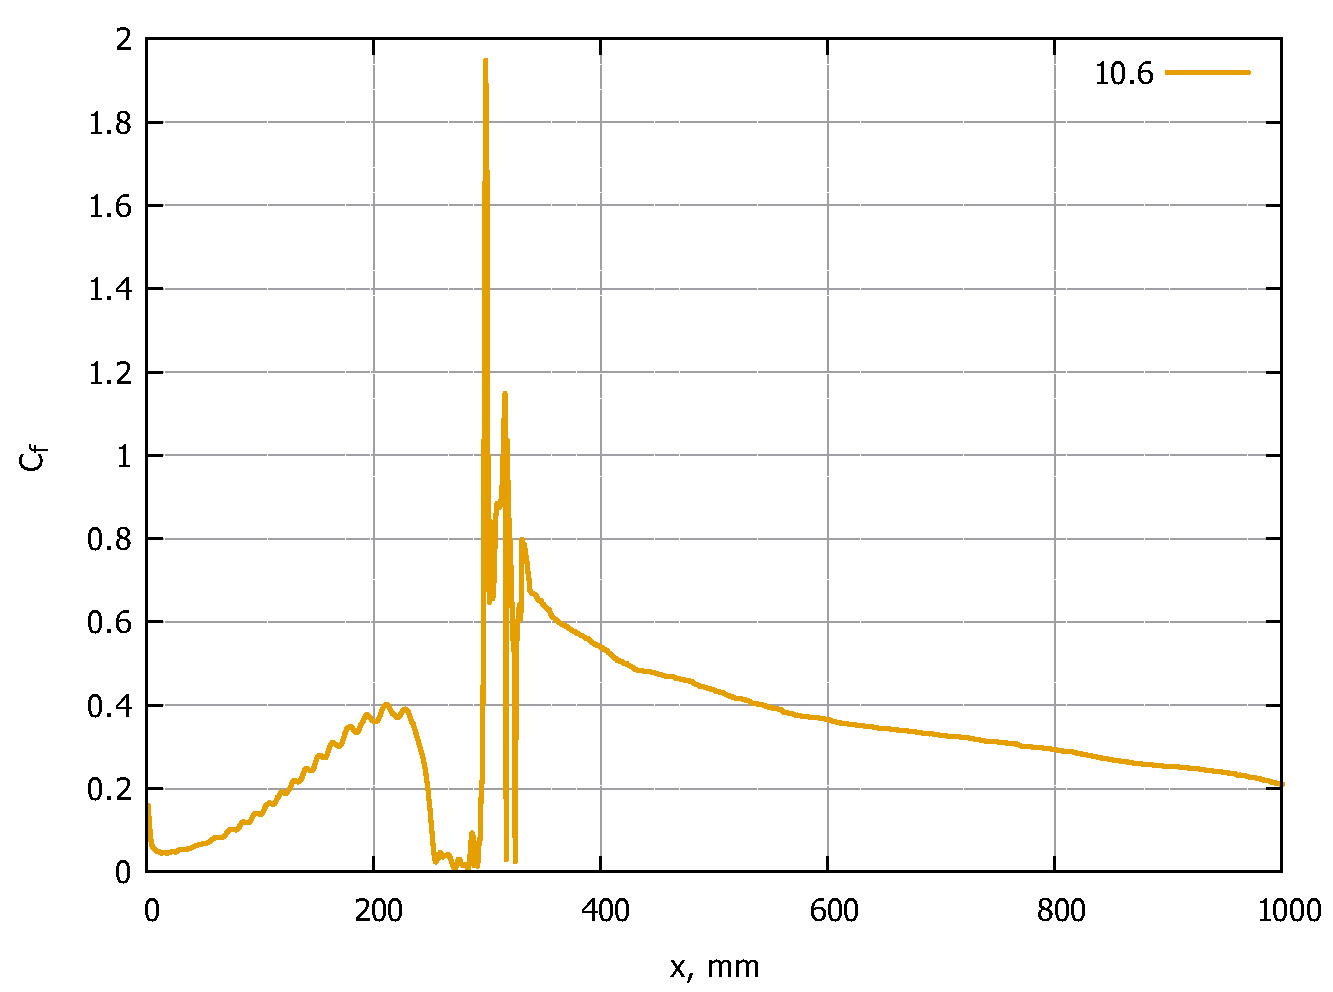
\includegraphics[width=1\linewidth]{../Assets/Cf-T1060-31m}
			\caption{t = 10.6 s}
			\label{fig:Cf-T1060-31m}
		\end{subfigure}
		\caption{Change in the friction coefficient along the length of the channel, z = -31 mm}
		\label{fig:cf-31m}
	\end{figure}
	\newpage
	In the left part of the channel, a similar change is observed as in the right. However, it is slightly less than in the previous case.
	\begin{figure}[H]
		\begin{subfigure}{.5\textwidth}
			\centering
			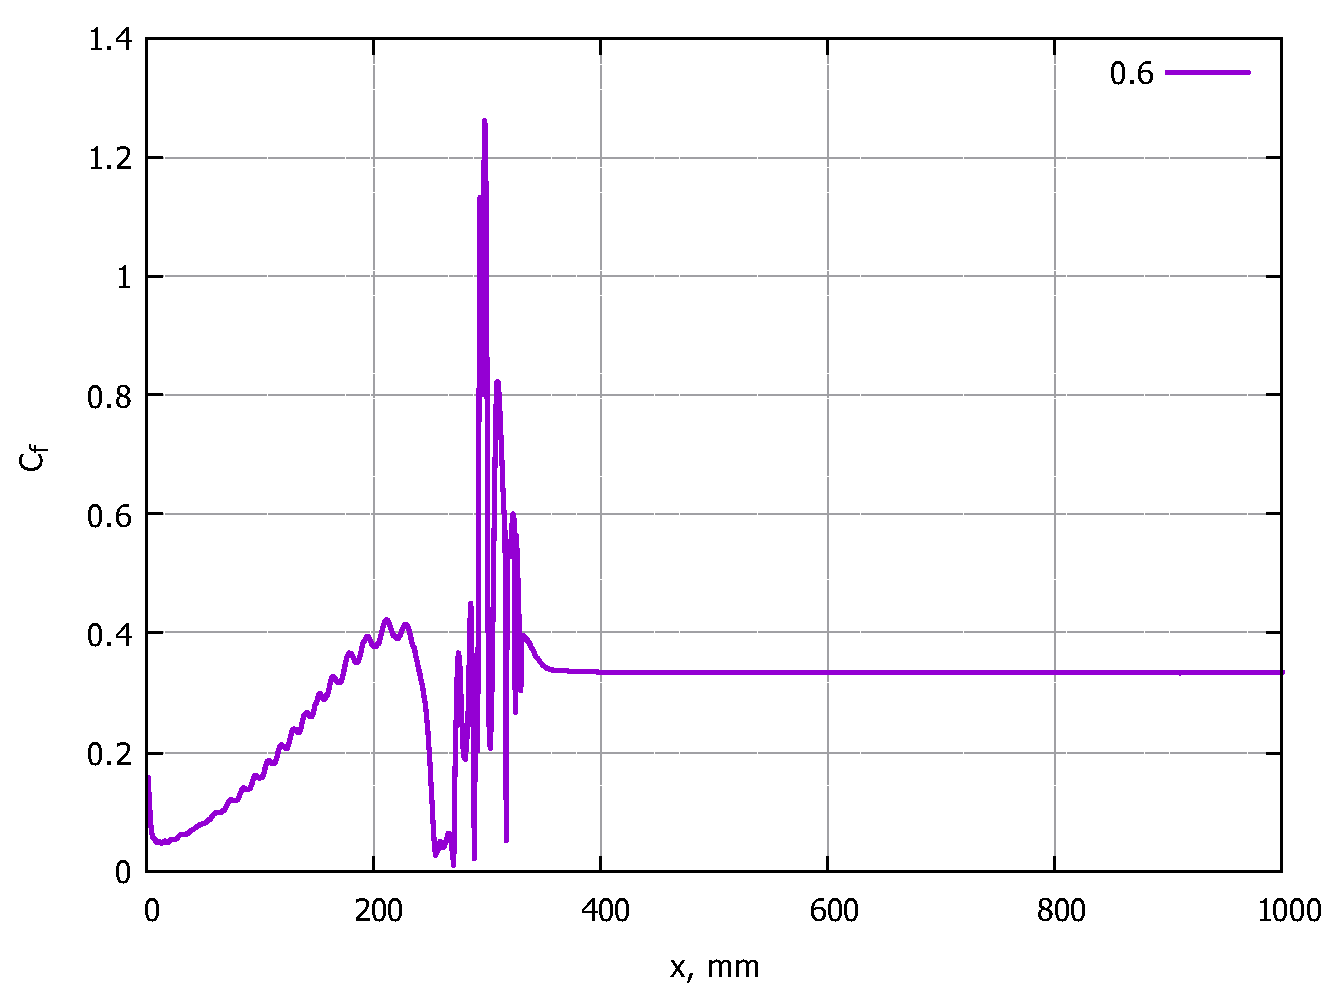
\includegraphics[width=1\linewidth]{../Assets/Cf-T06-31p}
			\caption{t = 0.6 s}
			\label{fig:Cf-T06-31p}
		\end{subfigure}%
		\begin{subfigure}{.5\textwidth}
			\centering
			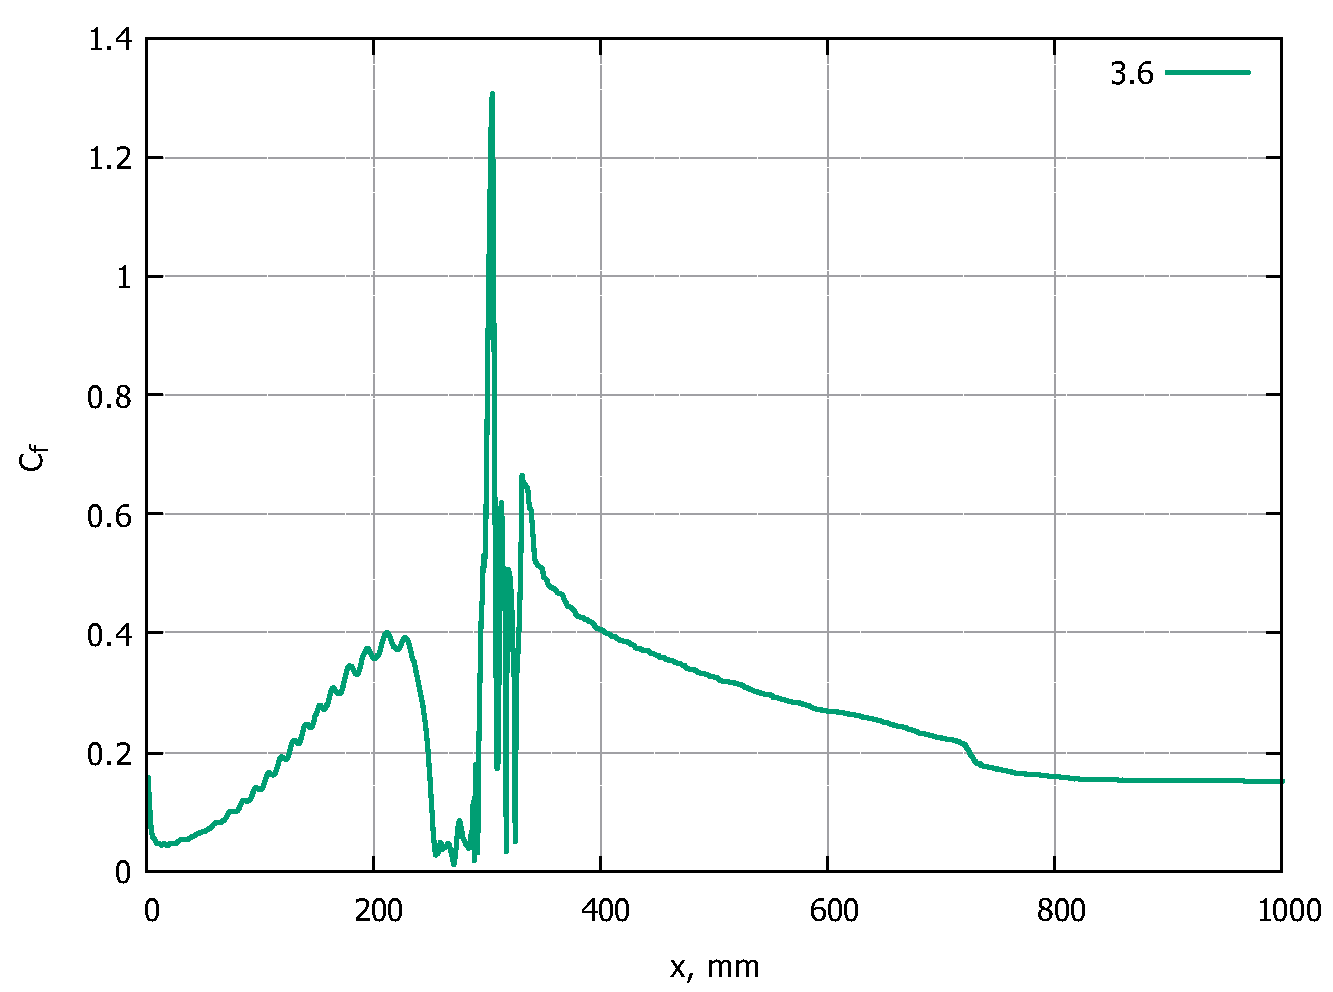
\includegraphics[width=1\linewidth]{../Assets/Cf-T360-31p}
			\caption{t = 3.6 s}
			\label{fig:Cf-T360-31p}
		\end{subfigure}
		\\
		\begin{subfigure}{.5\textwidth}
			\centering
			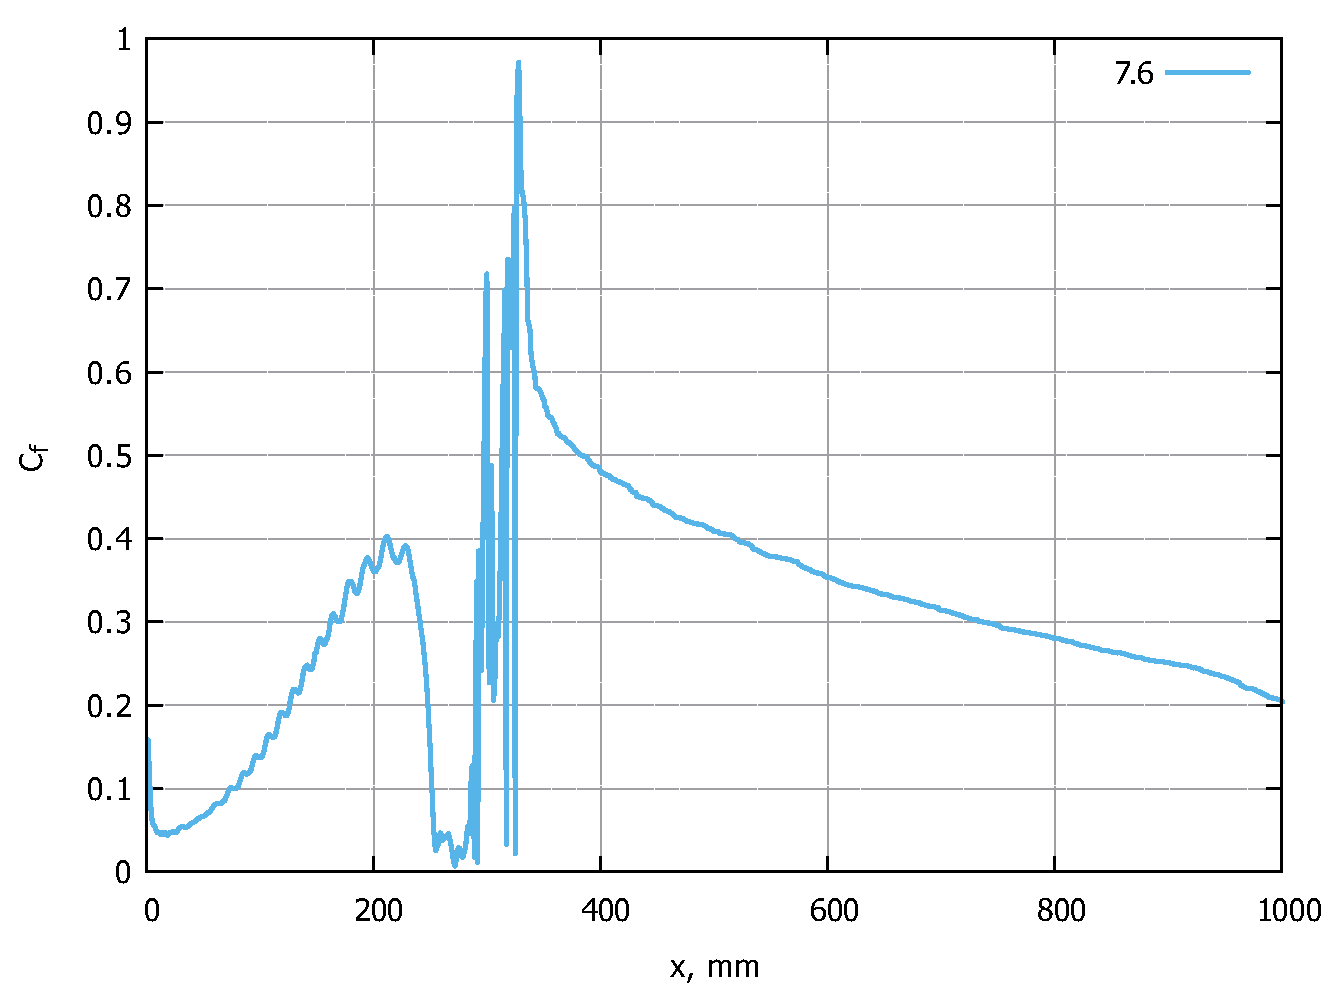
\includegraphics[width=1\linewidth]{../Assets/Cf-T760-31p}
			\caption{t = 7.6 s}
			\label{fig:Cf-T760-31p}
		\end{subfigure}%
		\begin{subfigure}{.5\textwidth}
			\centering
			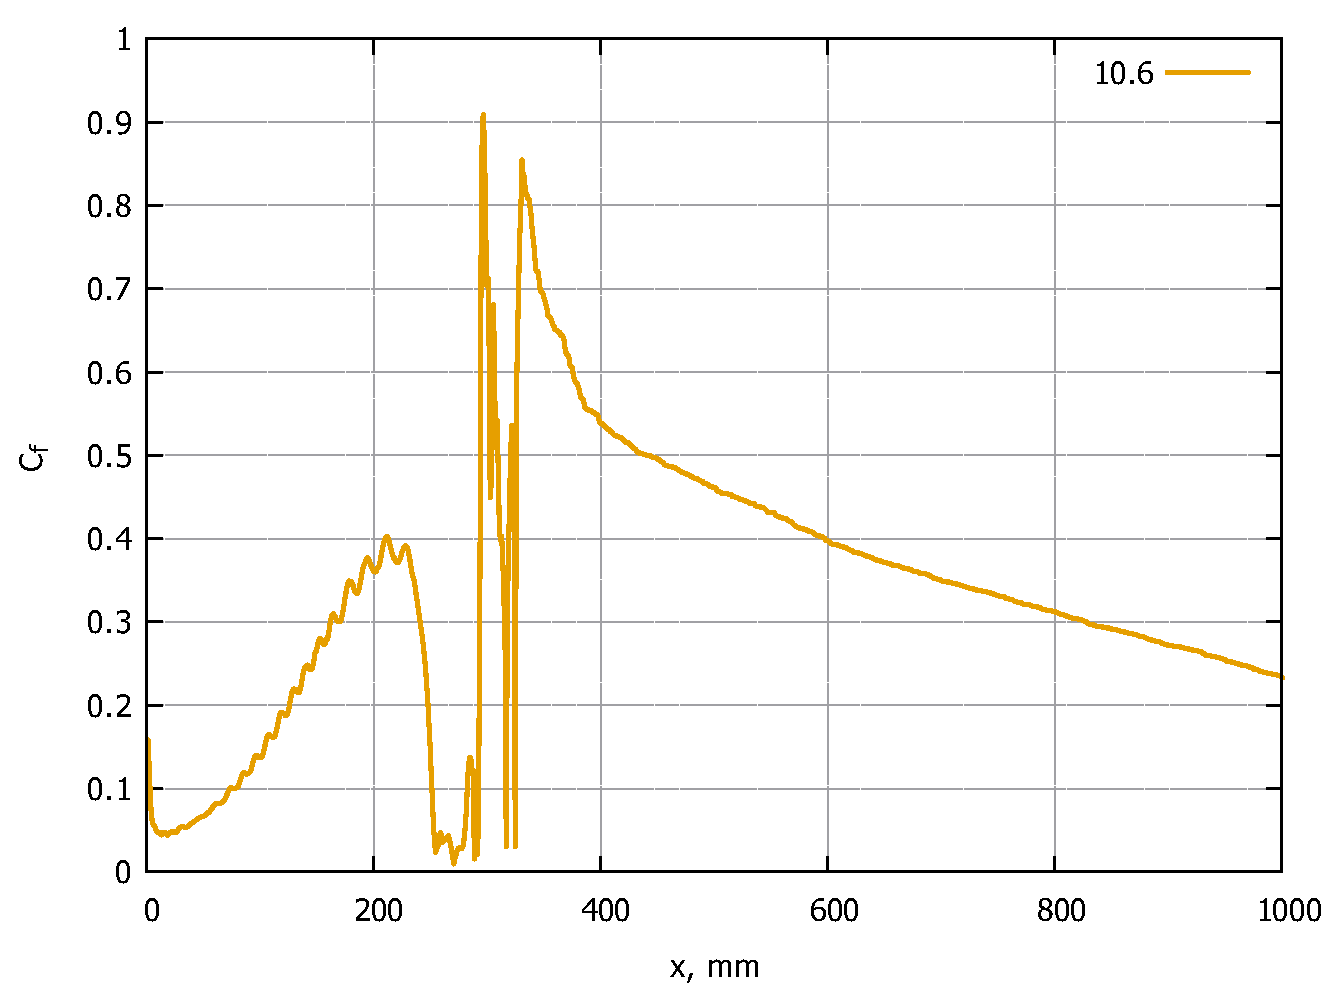
\includegraphics[width=1\linewidth]{../Assets/Cf-T1060-31p}
			\caption{t = 10.6 s}
			\label{fig:Cf-T1060-31p}
		\end{subfigure}
		\caption{Change in the friction coefficient along the length of the channel, z = 31 mm}
		\label{fig:cf-31p}
	\end{figure}
	\newpage
	Some combined variants by the plane. We can see, that coefficient changes more sharply for the section $z = -31$.
	\begin{figure}[H]
		\centering
		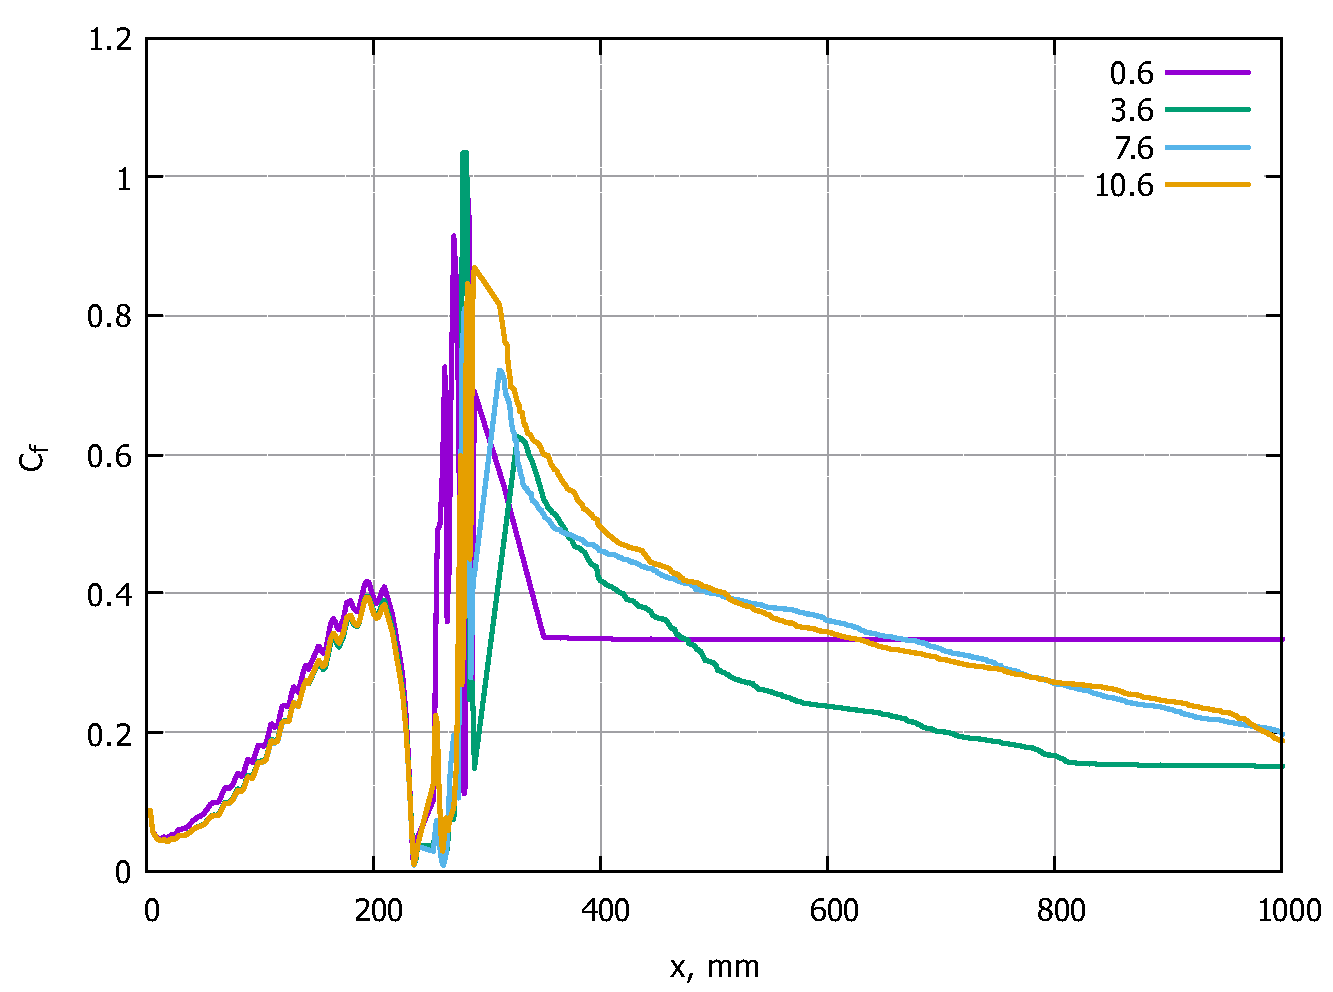
\includegraphics[width=0.7\linewidth]{../Assets/Cf-Tall}
		\caption{Change in the friction coefficient along the length of the channel, z = 0 mm}
		\label{fig:cf-tall}
	\end{figure}
	\begin{figure}[H]
		\centering
		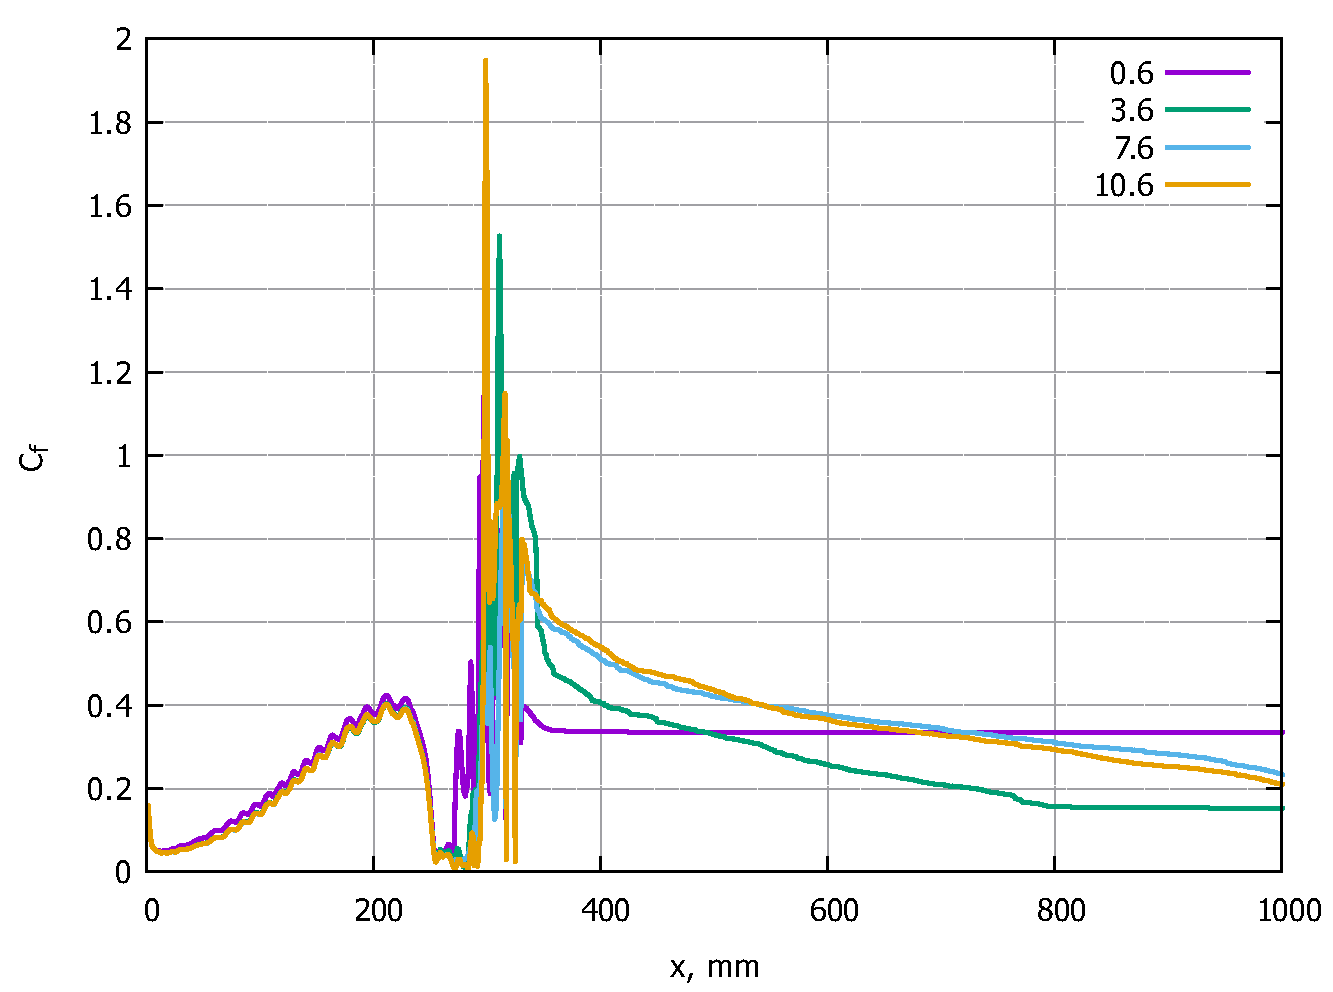
\includegraphics[width=0.7\linewidth]{../Assets/Cf-Tall-31m}
		\caption{Change in the friction coefficient along the length of the channel, z = -31 mm}
		\label{fig:cf-tall-31m}
	\end{figure}
	\begin{figure}[H]
		\centering
		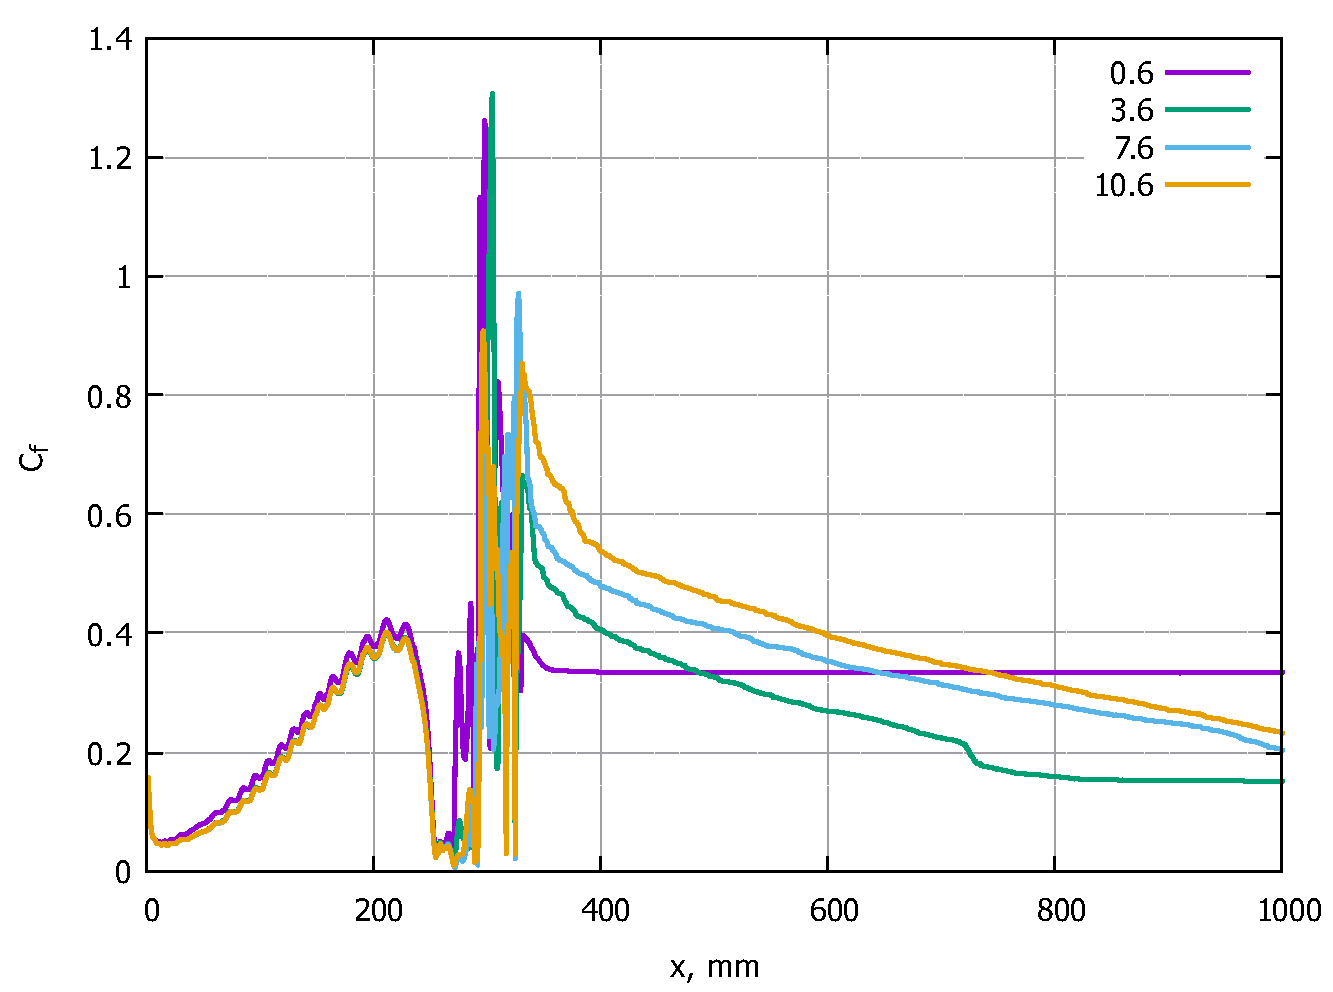
\includegraphics[width=0.7\linewidth]{../Assets/Cf-Tall-31p}
		\caption{Change in the friction coefficient along the length of the channel, z = 31 mm}
		\label{fig:cf-tall-31p}
	\end{figure}
	The previous statement is proved by the following set of plots. Also all sections has different changes from $z = 0$, because a lot of vortices generates near side walls than in the center of the channel.
	\begin{figure}[H]
		\centering
		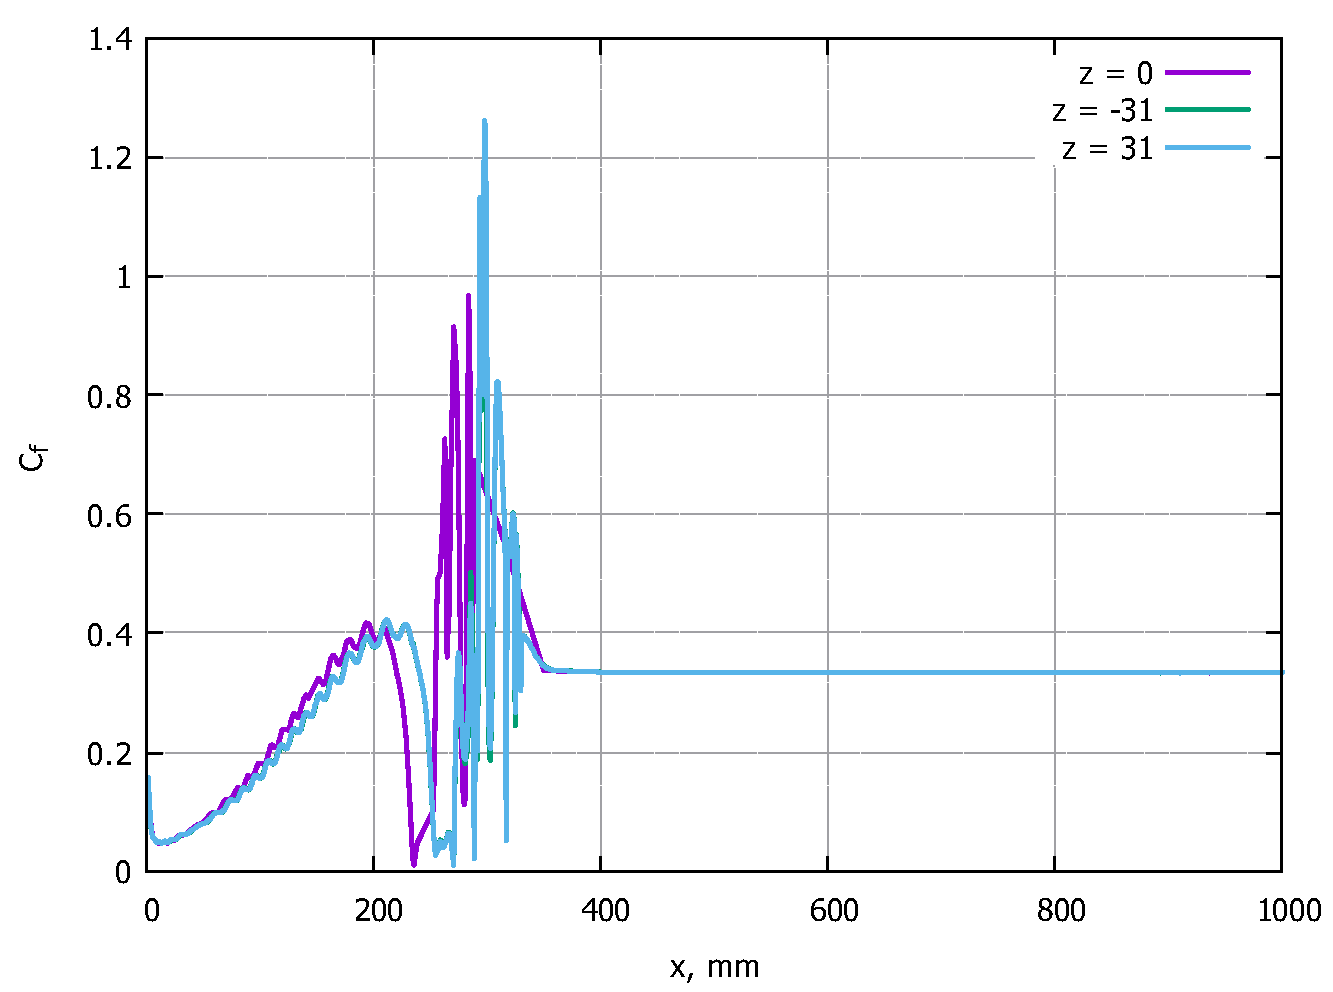
\includegraphics[width=0.7\linewidth]{../Assets/Cf-T06-all}
		\caption{Change in the friction coefficient along the length of the channel, t = 0.6 s}
		\label{fig:cf-t06-all}
	\end{figure}
	\begin{figure}[H]
		\centering
		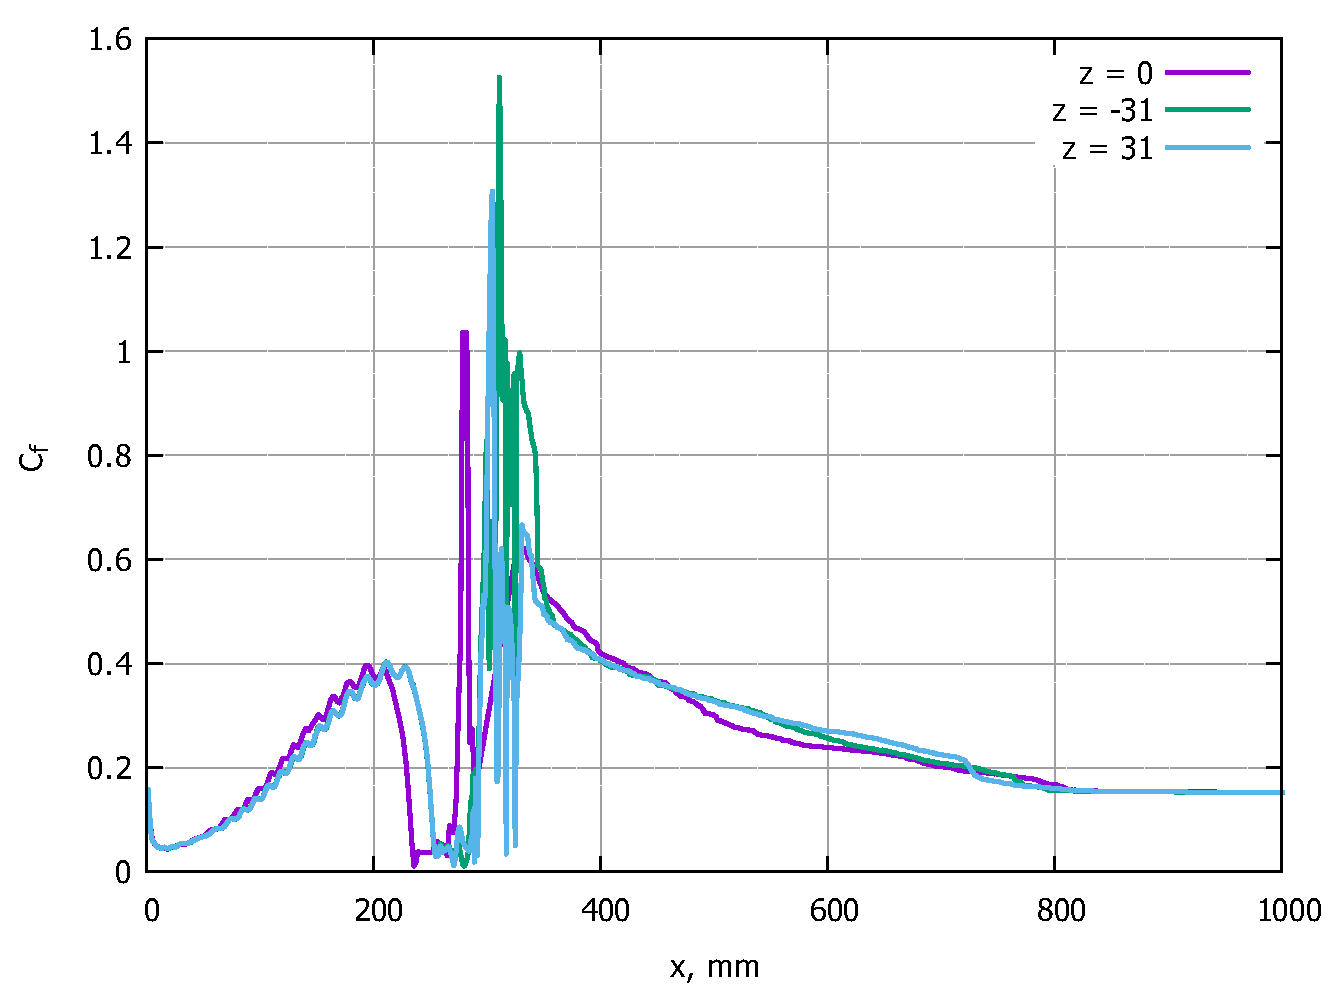
\includegraphics[width=0.7\linewidth]{../Assets/Cf-T360-all}
		\caption{Change in the friction coefficient along the length of the channel, t = 3.6 s}
		\label{fig:cf-t360-all}
	\end{figure}
	\begin{figure}[H]
		\centering
		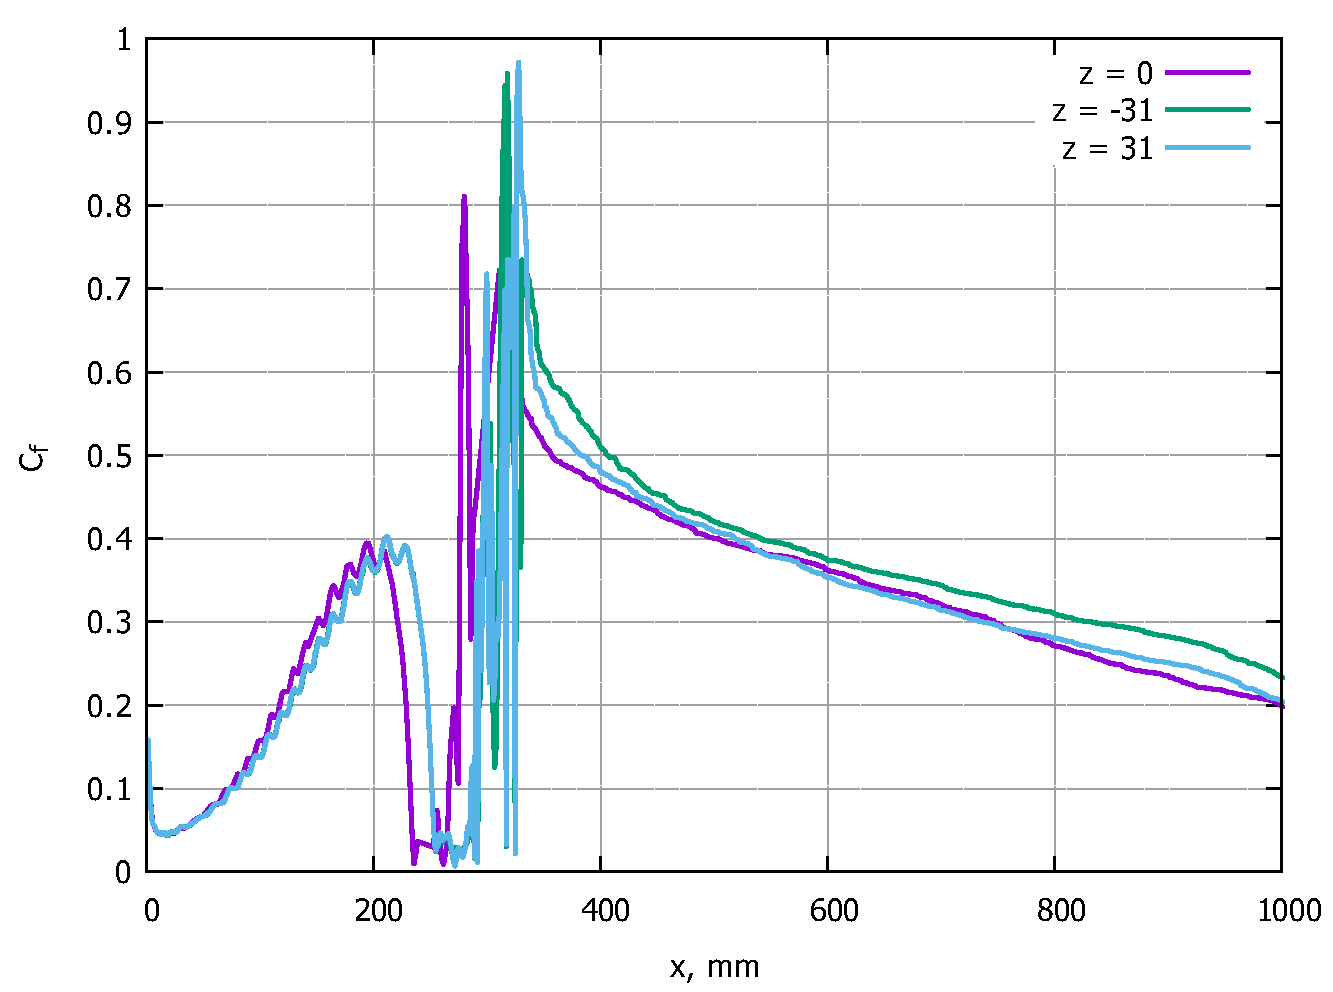
\includegraphics[width=0.7\linewidth]{../Assets/Cf-T760-all}
		\caption{Change in the friction coefficient along the length of the channel, t = 7.6 s}
		\label{fig:cf-t760-all}
	\end{figure}
	\begin{figure}[H]
		\centering
		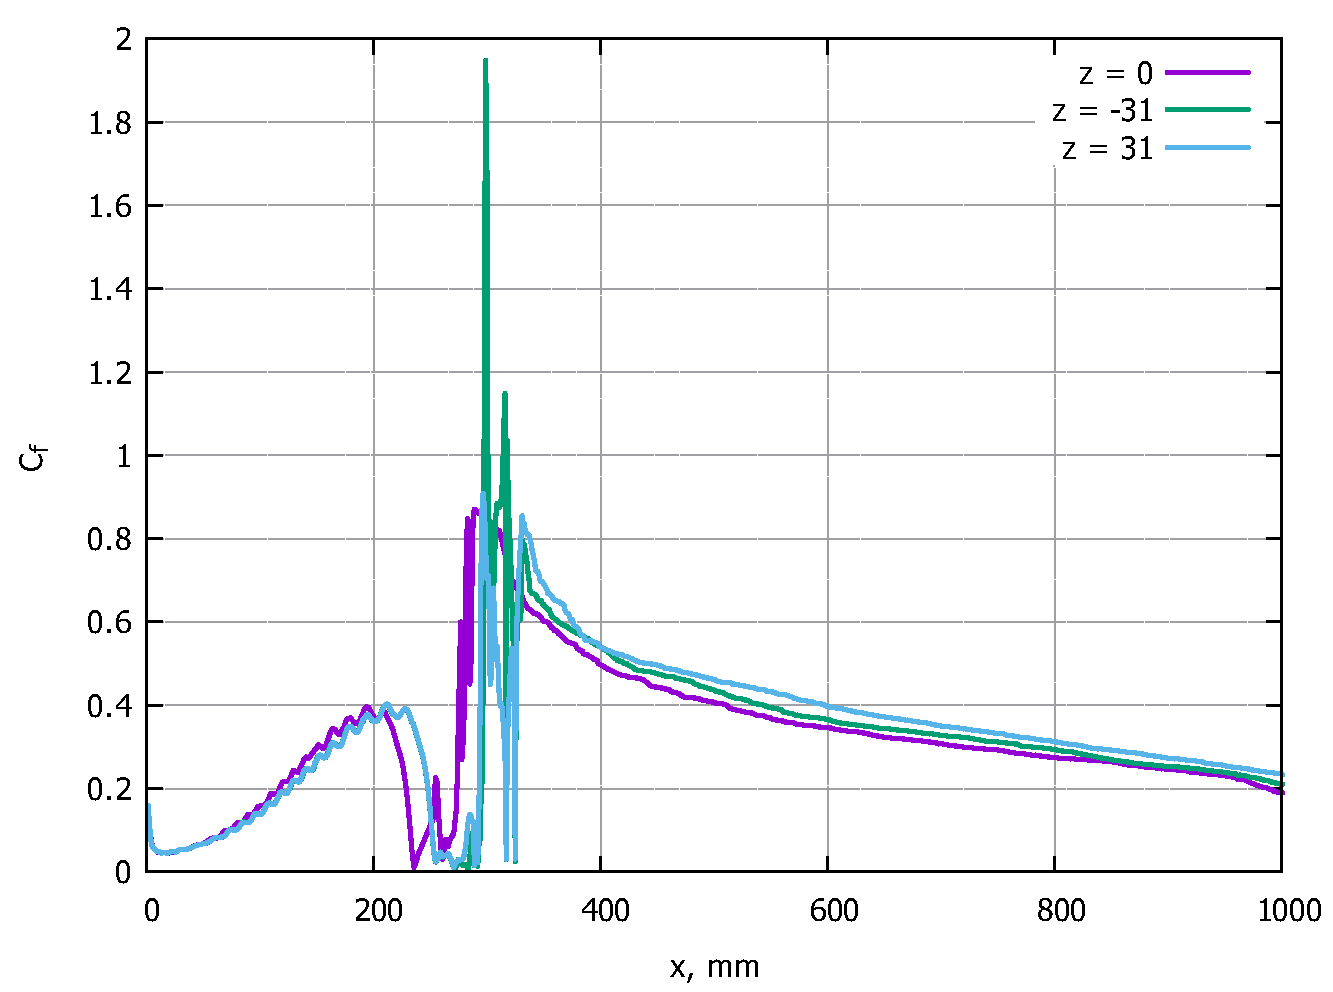
\includegraphics[width=0.7\linewidth]{../Assets/Cf-T1060-all}
		\caption{Change in the friction coefficient along the length of the channel, t = 10.6 s}
		\label{fig:cf-t1060-all}
	\end{figure}
\subsubsection{Q-criterion}
	There are various approaches to the visualization of vortex flows that use one or another definition of a vortex and criteria for its identification. The classification of visualization methods for vortex flows is carried out depending on how the vortex is defined (in the area or on the line), whether the method is invariant with respect to the transformation of the coordinate system, whether the approach is local or global\cite{Hunt1988}. One of these is the $Q$-criterion. It is determined by two components: the strain rate tensor $S$ and the rotation tensor $\Omega$.
	\begin{equation}
		S = \frac{1}{2}(\frac{\partial u_i}{\partial x_j} + \frac{\partial u_j}{\partial x_i}) \qquad \Omega = \frac{1}{2}(\frac{\partial u_i}{\partial x_j} - \frac{\partial u_j}{\partial x_i})
	\end{equation}
	The $Q$-criterion is defined as the second invariant of the velocity gradient tensor\cite{Wiebel2007}.
	\begin{equation}
		Q = \frac{1}{2}(||\Omega||^2 - ||S||^2)
	\end{equation}
	From this we can see that positive values of $Q$ indicate regions in the flow field where vorticity dominates, and negative values of $Q$ indicate regions where strain rate or viscous stress dominates. In addition, there are various versions of the $Q$ criterion in modified expressions that are used to describe different flow regions\cite{Berdahl1993,Chong1990}.
	\newpage
	Various areas of eddy formations are presented below. In the figure \ref{fig:q860-t16}, one can notice a clearly expressed structure of the formed vortex.
	\begin{figure}[H]
		\centering
		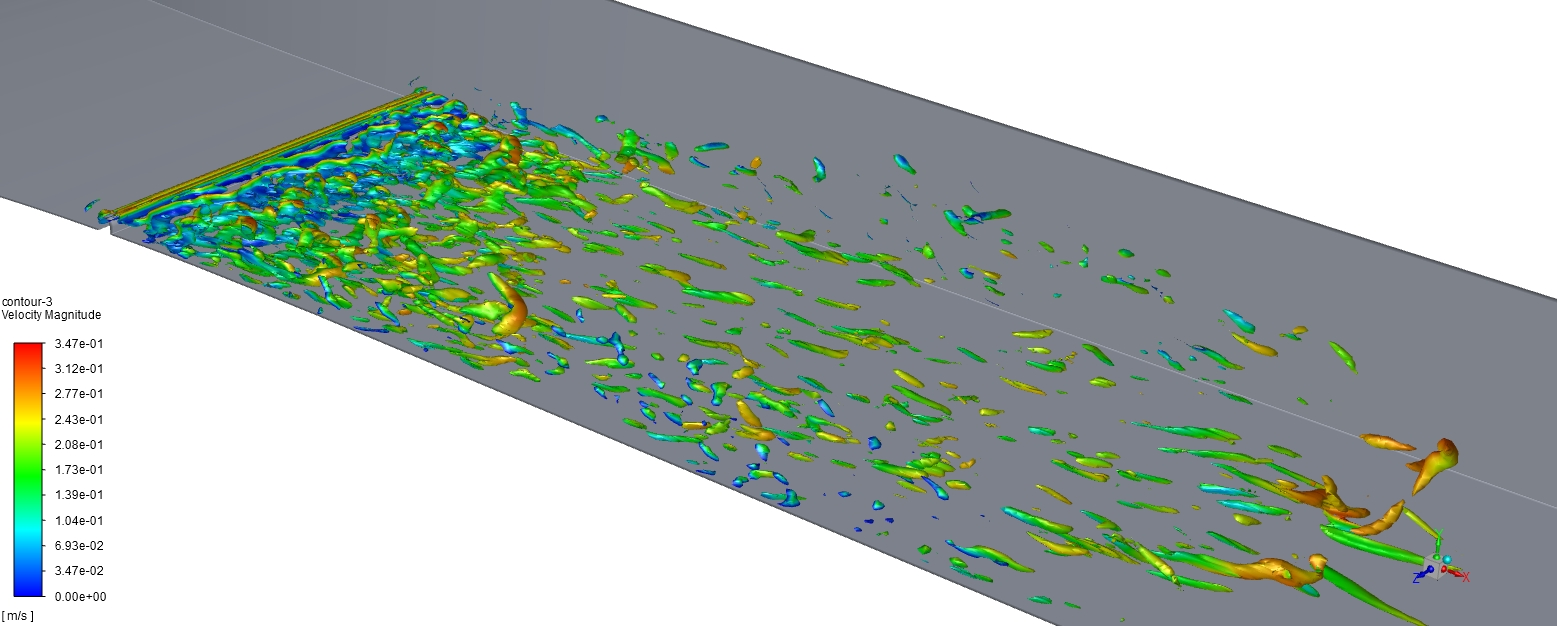
\includegraphics[width=1\linewidth]{../Assets/Q860-t16}
		\caption{Vortex structure at Q = 860 и t = 1.6 c}
		\label{fig:q860-t16}
	\end{figure}
	\begin{figure}[H]
		\centering
		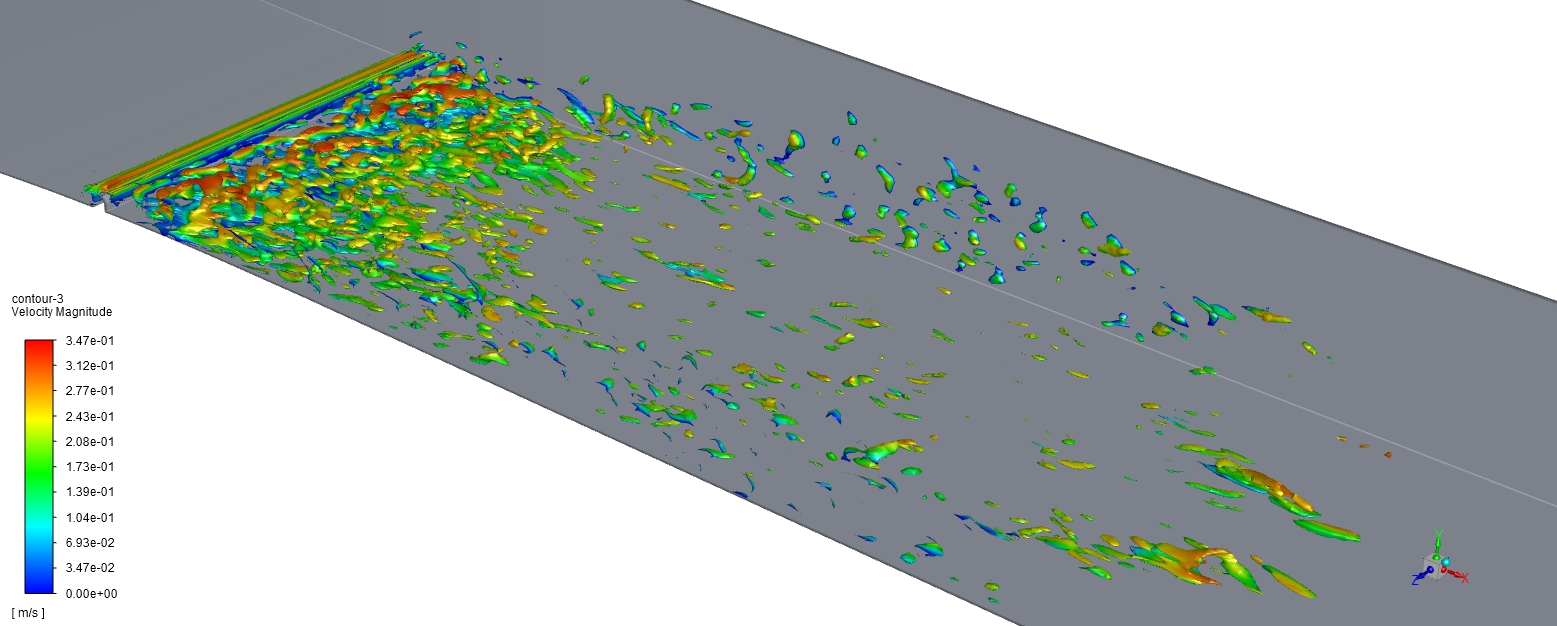
\includegraphics[width=1\linewidth]{../Assets/QM850-t16}
		\caption{Vortex structure at Q = -850 и t = 1.6 с}
		\label{fig:qm850-t16}
	\end{figure}
	So, if we downgrade the value of Q-criterion we can obtain a lot of small vortex structures due to their low speed.
	\nocite{KimW.W.1995,Agostini2014,Blackwelder1983,Abbas2017}